
%%%%%%%%%%%%%%%%%%%%%%%%%%%%%%%%%%%%%%%%%%%%%%%%%%%%%%%%%%%%%%%%%%%%%
\section{Calcul différentiel}
\subsection{Différentiabilité}


Pour une fonction $f : \Rr \to \Rr$ d'une seule variable, une autre façon d'écrire qu'elle est dérivable en $x_0$ est de vérifier qu'il existe $\ell \in \Rr$ tel que 
$$\lim_{h \rightarrow 0} \frac{f(x_0 + h) - f(x_0) - \ell \cdot h}{h} = 0.$$
Et on note ce $\ell$ par $f'(x_0)$, de sorte que l'on a 
$f(x_0+h) \simeq f(x_0) + f'(x_0)\cdot h$ (pour $h$ réel, assez petit).
Autrement dit, on approche l'application $h \mapsto f(x_0+h) - f(x_0)$
par une fonction linéaire $h \mapsto f'(x_0) \cdot h$.

\bigskip

Nous allons faire ce même travail en dimension supérieure.
\begin{definition}{}{}
	Soit $f : \Rr^n \to \Rr$. La fonction $f$ est \trouer{différentiable} en $x_0 \in \Rr^n$ s'il existe une application linéaire $\ell : \Rr^n \to \Rr$ telle que :
	$$\lim_{\|h\| \to 0}  \frac{f(x_0+ h) - f(x_0) - \ell(h)}{\|h\|} = 0$$
	L'application $\ell $ est la \trouer{différentielle} de $f$ en $x_0$ et se note $\dd f(x_0)$.
\end{definition}


Dans le cas des fonctions d'une variable, on a $\dd f(x_0) = f'(x_0)$ (et $\dd f(x_0)(h) = f'(x_0)\cdot h$).
Dans le cas des fonctions de plusieurs variables, on verra juste après comment écrire la différentielle à l'aide des dérivées partielles.
Noter que $\dd f(x_0)$ est une application de $\Rr^n$ vers $\Rr$ (comme $f$), et donc $\dd f(x_0)(h)$ est un réel (pour chaque $h\in\Rr^n$).


\bigskip

De même qu'en une variable, si une fonction est dérivable, alors elle est continue.
\begin{proposition}{}{diffcont}
	Si $f$ est différentiable en $x_0 \in \Rr^n$, alors $f$ est continue en $x_0$.
\end{proposition}

\begin{proof}
	Notons $g$ la fonction définie par $g(h)=\frac{f(x_0+h) - f(x_0) - \dd f(x_0)(h)}{\|h\|}$. Alors 
	$$f(x_0 + h)=f(x_0) + \dd f(x_0)(h) +\|h\|g(h)$$
	et il est clair que $\dd f(x_0)(h)$ et $\|h\|g(h)$ tendent vers $0$ lorsque $h$ tend vers le vecteur nul. Donc la limite de $f$ en $x_0$ existe et vaut $f(x_0)$, et ainsi $f$ est continue en $x_0$.
\end{proof}

\begin{exemple}{}{}
	Si $\ell : \Rr^n \to \Rr$ est linéaire, alors $\ell$ est différentiable et sa différentielle en tout point est l'application $\ell$ elle-même : pour tous $x_0 \in \Rr^n$ et $h \in \R^n$,
	$$
	\dd \ell (x_0) (h) = \ell(h).
	$$ 
\end{exemple}




%----------------------------------------------------
\subsection{Différentielle}


\begin{proposition}{}{differ}
	Si $f : \Rr^n \to \Rr$ est différentiable en $x_0 \in \Rr^n$, alors ses dérivées partielles existent et on a :
	$$
	\dd f(x_0)(h) = 
	h_1 \frac{\partial f}{\partial x_1}(x_0)  + \cdots + h_n \frac{\partial f}{\partial x_n}(x_0)  
	$$
	où $h = (h_1,\ldots,h_n)$.
\end{proposition}
En particulier, lorsqu'elle existe, la différentielle est unique.

\bigskip

Pour $f : \Rr^2 \to \Rr$ différentiable en $(x_0,y_0)$, la formule est :
\mybox{$
	\dd f(x_0,y_0)(h,k) = 
	h \frac{\partial f}{\partial x}(x_0,y_0) + 
	k \frac{\partial f}{\partial y}(x_0,y_0)
	$}

\begin{proof}
	Prouvons la formule pour deux variables.
	Soit $f : \Rr^2 \to \Rr$ différentiable en $(x_0,y_0) \in \Rr^2$.
	Soit $\ell(h,k) = ah + bk$ sa différentielle. Alors, par définition, lorsque $\|(h,k)\| \to 0$, on a :
	$$\frac{f(x_0+ h,y_0+k) - f(x_0,y_0) - \ell(h,k)}{\|(h,k)\|} \longrightarrow 0$$
	Pour $(h,k) = (t,0)$ avec $t>0$ et $t \to 0$, on a donc :
	$$\frac{f(x_0+ t,y_0) - f(x_0,y_0) - t\ell(1,0)}{t}
	= \frac{f(x_0+ t,y_0) - f(x_0,y_0)}{t} - \ell(1,0) \longrightarrow  0$$
	C'est exactement dire que 
	$$\frac{\partial f}{\partial x}(x_0,y_0) = \ell(1,0) = a.$$
	
	Avec $(h,k) = (0,t)$, on prouve de même que 
	$$\frac{\partial f}{\partial y}(x_0,y_0) = \ell(0,1) = b.$$
	
	Ainsi,
	$$\ell(h,k) = h \frac{\partial f}{\partial x}(x_0,y_0) +
	k \frac{\partial f}{\partial y}(x_0,y_0).$$
\end{proof}




Pour montrer qu'une fonction est différentiable, on peut utiliser que la somme, le produit, l'inverse (d'une fonction ne s'annulant pas) et la composition de fonctions différentiables est différentiable. Sinon, il faut revenir à la définition. Par exemple, pour $f : \Rr^2 \to \Rr$ : 
\begin{enumerate}
	\item tout d'abord, on calcule les dérivées partielles 
	$\frac{\partial f}{\partial x}(x_0,y_0)$ et  $\frac{\partial f}{\partial y}(x_0,y_0)$, 
	
	\item on écrit le  candidat à être la différentielle $
	\ell(h,k) = 
	h \frac{\partial f}{\partial x}(x_0,y_0) + 
	k \frac{\partial f}{\partial y}(x_0,y_0)
	$,
	
	\item il faut enfin prouver la limite, lorsque $\|(h,k)\| \to 0$ :
	$$\frac{f(x_0+ h,y_0+k) - f(x_0,y_0) - \ell(h,k)}{\|(h,k)\|} \longrightarrow  0.$$
	
\end{enumerate}




\begin{exemple}{}{}
	\'Etudier la différentiabilité en tout point de la fonction $f$ définie par
	$$f(x,y)= x-3y + \frac{x^4}{x^2+y^2}\quad\mbox{ si }(x,y)\neq (0,0)\qquad \text{ et }\quad f(0,0)=0.$$
	
	
	\bigskip
	\emph{Solution.}
	
	\begin{itemize}
		\item En dehors de $(0,0)$, la fonction $f$ est différentiable, car $f$ est une somme, produit, inverse de fonctions différentiables (car $x^2+y^2$ ne s'annule qu'à l'origine).
		
		\item En $(0,0)$, il faut étudier la différentiabilité à la main.
		\begin{itemize}
			\item Dérivée partielle par rapport à $x$ :
			
			$$\frac{\partial f}{\partial x}(0,0) = \lim _{h\to 0}\frac{f(h,0)-f(0,0)}{h}=\lim _{h\to 0}\frac{h+h^2}{h}=1$$
			
			
			\item Dérivée partielle par rapport à $y$ :
			
			$$\frac{\partial f}{\partial y}(0,0) = \lim _{k\to 0}\frac{f(0,k)-f(0,0)}{k}=\lim_{k\to 0}\frac{-3k}{k}=-3$$
			
			\item Le candidat à être la différentielle est donc :
			$$\ell(h,k) = 
			h \frac{\partial f}{\partial x}(0,0) + 
			k \frac{\partial f}{\partial y}(0,0)
			= h-3k$$
			
			\item On calcule :
			$$0 \le \frac{f(0+h,0+k) - f(0,0) - \ell(h,k)}{\sqrt{h^2+k^2}}
			=  \frac{h^4}{(h^2+k^2)^{\frac{3}{2}}}
			\le \frac{h^4}{|h|^3}
			=|h|
			\xrightarrow[(h,k)\to(0,0)]{} 0
			.$$    
			
		\end{itemize}
		
		Donc $f$ est différentiable au point $(0,0)$ et $\dd f (0,0)(h,k) = h-3k$.
		
	\end{itemize}
	
\end{exemple}

%----------------------------------------------------
\subsection{Lien avec les dérivées partielles}


\bigskip
\evidence{Dérivées partielles.}

On a vu dans la proposition \ref{pr:differ} que si $f : \Rr^2 \to \Rr$ est différentiable en $(x_0,y_0)$, alors
$$\dd f (x_0,y_0) (1,0) = \frac{\partial f}{\partial x}(x_0,y_0)
\qquad \text{ et } \qquad
\dd f (x_0,y_0) (0,1) = \frac{\partial f}{\partial y}(x_0,y_0).$$

En toute dimension, pour $f : \Rr^n \to \Rr$ différentiable en $x_0 \in \Rr^n$, et $e_i$ le $i$-ème vecteur de la base canonique :
$$\dd f (x_0) (e_i) = \frac{\partial f}{\partial x_i}(x_0).$$



\bigskip
\evidence{Dérivée directionnelle.}

Plus généralement, si $f : \Rr^n \to \Rr$ est différentiable en $x_0 \in \Rr^n$, alors $\dd f (x_0) (v) = D_v f(x_0)$.
Pour $f : \Rr^2 \to \Rr$, cela signifie que si $v=(h,k)$, alors :
\mybox{$D_{(h,k)} f(x_0,y_0) = h \frac{\partial f}{\partial x}(x_0,y_0) +
	k \frac{\partial f}{\partial y}(x_0,y_0)$}

Si $f$ n'est pas différentiable, cette formule peut être fausse.

\bigskip
\evidence{Gradient.}

Le gradient est une autre façon de coder la différentielle.
Le \trouer{gradient} de $f$ en $x_0$ est le vecteur
$$\grad f (x_0) =
\begin{pmatrix}
	\dfrac{\partial f}{\partial x_{1}} (x_0)\\
	\vdots \\
	\dfrac{\partial f}{\partial x_n}(x_0)
\end{pmatrix}.$$

Si $f$ est différentiable en $x_0$, alors
$$\dd f (x_0) (v) = \langle \grad f (x_0) \mid v \rangle,$$
où $\langle u \mid v \rangle$ est le produit scalaire de $u$ et $v$.

Nous reviendrons en détail sur le gradient et ses applications dans le chapitre \og{}Gradient -- Théorème des accroissements finis\fg{}.


\bigskip
\evidence{Résumé.}

Lorsque $f$ est différentiable alors la différentielle, la dérivée directionnelle, et le gradient encodent la même information et sont reliés  
par les formules :
\mybox{$\displaystyle
	D_v f(x_0) = \dd f (x_0) (v) = \langle \grad f (x_0) \mid v \rangle
	$}



\begin{exemple}{}{}
	Soit $f$ la fonction définie par 
	$$f(x,y) =  \ln(1+x+y^2).$$
	
	\begin{enumerate}
		\item Déterminer le domaine de définition $U$ de $f$.
		\item Calculer les dérivées partielles de $f$.
		\item Montrer que $f$ est différentiable sur $U$.
		\item Calculer le gradient de $f$ en $(0,1)$ et exprimer la différentielle en ce point.
		\item Calculer la dérivée directionnelle de $f$ en $(0,1)$ suivant le vecteur $(2,1)$.
	\end{enumerate}
	
	\bigskip
	\emph{Solution.}
	
	
	
	
	
	\begin{enumerate}
		\item On a $U = \big\{ (x,y) \in \Rr^2 \mid 1+x+y^2>0 \big\}$.
		
		\myfigure{1}{
			\tikzinput{fig-calculdiff-02}
		}
		
		\item Les dérivées partielles sont :
		$$\frac{\partial f}{\partial x}(x,y) = \frac{1}{1+x+y^2} \qquad\qquad
		\frac{\partial f}{\partial y}(x,y) = \frac{2y}{1+x+y^2}$$
		
		
		\item $f$ est différentiable sur $U$ comme somme, produit et composée de fonctions différentiables.
		
		\item Le gradient s'obtient directement à partir des dérivées partielles :
		$$\grad f (0,1) = \begin{pmatrix} \dfrac{\partial f}{\partial x}(0,1) \\\dfrac{\partial f}{\partial y}(0,1) \end{pmatrix} = 
		\begin{pmatrix} \frac12 \\ 1 \end{pmatrix}$$
		
		La différentielle en ce point $\dd f(0,1) : \Rr^2 \to \Rr$ est l'application linéaire définie par 
		$$\dd f(0,1)(h,k) = \langle \grad f (0,1) \mid (h,k) \rangle = \frac12h +k.$$
		
		\item Comme $f$ est différentiable, la dérivée directionnelle est simplement la combinaison linéaire des dérivées partielles :
		$$D_{(2,1)} f(0,1) = 2\times \frac{\partial f}{\partial x}(0,1)+1\times
		\frac{\partial f}{\partial y}(0,1) = 2$$
		On aurait aussi pu faire le calcul via la formule $D_{(2,1)} f(0,1) = \dd f(0,1)(2,1)$.
	\end{enumerate} 
	
\end{exemple}



%----------------------------------------------------
\paragraph{Exercices :}
	\begin{enumerate}
		\item Soit $g : \Rr \to \Rr$ dérivable. Soit $f : \Rr^2 \to \Rr$ définie par $f(x,y)= g(x+y)$. Montrer que $f$ est différentiable et que
		$\dd f (x_0,y_0)(h,k) = g'(x_0+y_0)h + g'(x_0+y_0)k$.
		
		\item Soit $f(x,y) = 2xy-7x+8y$. En utilisant la définition, montrer que $f$ est différentiable et calculer sa différentielle.
		
		\item Soit $f$ définie par $f(x,y) = ye^{x/y}$. Trouver le domaine de définition $U$ de $f$. Montrer que $f$ est différentiable sur $U$. Calculer ses dérivées partielles. Calculer la dérivée directionnelle de $f$ en $(4,2)$ suivant le vecteur $v = (-1,1)$.
		
	\end{enumerate}






%%%%%%%%%%%%%%%%%%%%%%%%%%%%%%%%%%%%%%%%%%%%%%%%%%%%%
\section{Fonctions de classe $\mathcal{C}^1$}

Dans la pratique, les fonctions seront souvent de classe $\mathcal{C}^1$, ce qui implique la différentiabilité, et est plus facile à vérifier. 


%----------------------------------------------------
\subsection{Définition}

\begin{definition}{}{}
	Soit $f: \Rr^n \to \Rr$. On dit que $f$ est de \trouer{classe $\mathcal{C}^1$} si les dérivées partielles $\frac{\partial f}{\partial x_i}$
	existent et sont continues (pour $i=1,\ldots,n$).
\end{definition}

On peut bien sûr limiter la définition à un ouvert. Par exemple, si $U$ un ouvert de $\Rr^2$, $f : U \to \Rr$ sera de classe $\mathcal{C}^1$ sur $U$ si $\frac{\partial f}{\partial x}$ et $\frac{\partial f}{\partial y}$ existent et sont continues sur $U$.


\begin{theoreme}{Condition suffisante de différentiabilité}{foncc1}
	Si $f$ est de classe $\mathcal{C}^1$, alors $f$ est différentiable.
\end{theoreme}

Une autre façon de dire que $f$ est différentiable est de dire que $f$ admet un \trouer{développement limité à l'ordre~$1$}. Pour $f : \Rr^2 \to \Rr$, si $f$ est différentiable au point $(x_0,y_0)$, alors
$$f(x_0+h,y_0+k)=f(x_0,y_0)+h\frac{\partial f}{\partial x}(x_0,y_0)+k\frac{\partial f}{\partial y}(x_0,y_0)+o\left(\|(h,k)\|\right).$$

\bigskip

On rappelle la notation \og{}petit o\fg{}.

\textbf{Notation.} Soit $g :\Rr^2\to \Rr$ une fonction définie au voisinage de $(0,0)$. On dit que $g$ est \trouer{négligeable} par rapport à $\|(x,y)\|^n$ au voisinage de $(0,0)$ et on note $g=o\left(\|(x,y)\|^n\right)$ si 
$$\lim_{(x,y)\to(0,0)}\frac{g(x,y)}{\|(x,y)\|^n}=0.$$

\begin{exemple}{}{}
	Soit $f : \Rr^2 \to \Rr$ définie par $f(x,y)=\sin x \cdot e ^{2y}$.
	
	\begin{itemize}
		\item On a : $\frac{\partial f}{\partial x}(x,y)=\cos x \cdot e ^{2y}$ et $\frac{\partial f}{\partial y}(x,y)=2\sin x \cdot e ^{2y}$. Les deux dérivées partielles existent et sont continues donc $f$ est de classe $\mathcal{C}^1$ sur tout $\Rr^2$. 
		
		\item En particulier, $f$ est différentiable en tout point $(x_0,y_0) \in \Rr^2$ et 
		$$\dd f (x_0,y_0)(h,k) = h\cos x_0 e ^{2y_0}+2k\sin x_0 e ^{2y_0}.$$
		
		\item Par exemple, pour $(x_0,y_0) = (\frac\pi6,1)$, on a le développement limité :
		$$f(\tfrac\pi6+h,1+k) = f(\tfrac\pi6,1) + 
		h\frac{\partial f}{\partial x}(\tfrac\pi6,1)+
		k \frac{\partial f}{\partial y}(\tfrac\pi6,1) + o\left(\|(h,k)\|\right)$$
		Ainsi :
		$$f(\tfrac\pi6+h,1+k) = \frac{1}{2}e^2 + \frac{\sqrt3}{2}e^2h + 
		e^2k + \epsilon(h,k)\sqrt{h^2+k^2}$$
		où $\epsilon(h,k) \to 0$ lorsque $(h,k) \to (0,0)$. 
	\end{itemize}
	
\end{exemple}



\begin{proof}
	Soit $f$ une fonction de classe $\mathcal{C}^1$ au voisinage du point $(x_0,y_0)$ : elle admet donc des dérivées partielles continues au voisinage de $(x_0,y_0)$. 
	
	
	Pour $(h,k)\in \Rr^2$, on a
	$$f(x_0+h,y_0+k)-f(x_0,y_0)=\big[f(x_0+h,y_0)-f(x_0,y_0)\big]
	+\big[f(x_0+h,y_0+k)-f(x_0+h,y_0)\big].$$
	
	La fonction $x\mapsto f(x,y_0)$ est dérivable en $x_0$, donc $$f(x_0+h,y_0)-f(x_0,y_0)=h\frac{\partial f}{\partial x}(x_0,y_0)+ h\epsilon_1(h)$$
	avec $\lim _{h\to 0}\epsilon _1(h)=0$.
	
	Fixons $h$ : la fonction $y\mapsto f(x_0+h,y)$ est dérivable autour de $y_0$. Appliquons le théorème des accroissements finis à cette fonction d'une variable sur l'intervalle $[y_0,y_0+k]$ ; il existe donc $\ell \in {}]0,k[$ tel que 
	$$f(x_0+h,y_0+k)-f(x_0+h,y_0) = k \frac{\partial f}{\partial y}(x_0+h,y_0+\ell).$$
	Le réel $\ell$ dépend de $k$ et de $h$ et tend vers $0$ lorsque $k$ tend vers $0$ (uniformément en $h$).
	Or, $\frac{\partial f}{\partial y}$ est continue au point $(x_0,y_0)$, donc $\frac{\partial f}{\partial y}(x_0+h,y_0+\ell)=\frac{\partial f}{\partial y}(x_0,y_0)+\epsilon_2(h,k)$ avec $\lim _{(h,k)\to (0,0)}\epsilon_2(h,k)=0$,
	d'où
	$$f(x_0+h,y_0+k)-f(x_0+h,y_0)=k\frac{\partial f}{\partial y}(x_0,y_0)+k\epsilon _2(h,k).$$
	
	Ainsi, 
	$$f(x_0+h,y_0+k)-f(x_0,y_0)=h\frac{\partial f}{\partial x}(x_0,y_0)+k\frac{\partial f}{\partial y}(x_0,y_0)+h\epsilon _1(h)+k\epsilon _2(h,k).$$
	
	Or
	$$\frac{|h\epsilon _1(h)+k\epsilon _2(h,k)|}{\|(h,k)\|}\le |\epsilon _1(h)|+|\epsilon _2(h,k)| \xrightarrow[(h,k)\to(0,0)]{} 0,$$
	donc
	$$f(x_0+h,y_0+k)-f(x_0,y_0)=\dd f (x_0,y_0)(h,k)+o\left(\|(h,k)\|\right).$$
	Ainsi $f$ admet un développement limité d'ordre $1$ au point $(x_0,y_0)$, autrement dit $f$ est différentiable en ce point.
\end{proof}



%----------------------------------------------------
\subsection{Résumé}


\myfigure{1}{
	\tikzinput{fig-calculdiff-01}
}

\begin{itemize}
	\item Les équivalences sont issues des définitions.
	\item Les implications viennent du théorème \ref{th:foncc1}, de la proposition \ref{pr:diffcont} et de la proposition \ref{pr:differ}.
	\item Les implications inverses sont fausses : voir les exemples ci-dessous.
\end{itemize}



%----------------------------------------------------
\subsection{Contre-exemples}


Dans cette partie, on justifie que les énoncés précédents ne peuvent pas être améliorés. Cette section peut être passée en première lecture.


\bigskip


Si $f$ est différentiable, alors $f$ est continue. La réciproque est fausse, comme le prouve l'exemple suivant.

\begin{exemple}{}{}
	Soit $f : \Rr^2 \to \Rr$ définie par $f(x,y) = |x+y|$.
	Alors $f$ est continue (comme somme et composée de fonctions continues), mais n'est pas différentiable. Par exemple, $\frac{\partial f}{\partial x}$ n'est pas définie en $(0,0)$, car 
	$$\frac{f(0+h,0)-f(0,0)}{h} = \frac{|h|}{h}$$
	n'a pas de limite lorsque $h \to 0$. (Plus précisément, c'est $+1$ pour les $h>0$ et $-1$ pour les $h<0$.) Donc $f$ n'est pas différentiable en $(0,0)$.
	
	
	\begin{center}
		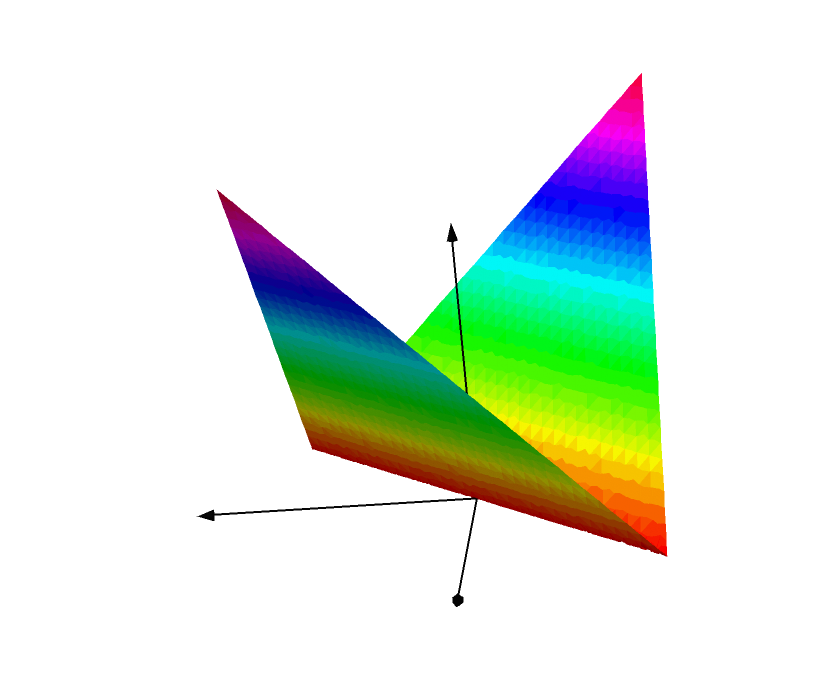
\includegraphics[scale=0.3]{figures/fig-calculdiff-03}
	\end{center}
	
	
	Sur la figure du graphe de $f$, on devine que, en tout point de la droite $(y=-x)$, $f$ n'est pas différentiable.
\end{exemple}


\bigskip



Si $f$ est différentiable, alors $f$ admet des dérivées partielles et des dérivées directionnelles dans toutes les directions. La réciproque est fausse, comme le prouve l'exemple suivant.

\begin{exemple}{}{}
	Soit $f:\Rr^2\to \Rr$ la fonction définie par
	$$f(x,y)=\frac{y^3}{\sqrt{x^2+y^4}}\quad \text{ si }(x,y)\neq (0,0)\qquad \text{ et }\quad f(0,0)=0.$$
	Montrer que $f$ admet une dérivée directionnelle suivant tout vecteur non nul au point $(0,0)$, mais qu'elle n'y est pas différentiable.
	
	
	\bigskip
	\emph{Solution.}
	
	\begin{enumerate}
		\item Soit $v=(h,k)\neq (0,0)$.
		\begin{itemize}
			\item Si $h=0$, on a $\displaystyle \frac{f(t \cdot v)-f(0,0)}{t}=\frac{f(0,tk)}{t}=k$.
			\item Si $h\neq 0$, on a $\displaystyle \left\vert \frac{f(t\cdot v)-f(0,0)}{t}\right\vert= \left\vert \frac{k^3t^2}{\sqrt{h^2t^2+h^4t^4}}\right\vert \le \left\vert \frac{k^3}{h}\right\vert |t|\underset{t\to 0}{\longrightarrow} 0$.
		\end{itemize}
		Ainsi, $\displaystyle D_{v}f(0,0)=
		\left\{
		\begin{array}{ccc}
			k&\text{ si }& h =0, \\ 
			0&\text{ si }& h\neq 0. 
		\end{array}\right.$
		
		
		\item Avec $v=(1,0)$, on aura $\frac{\partial f}{\partial x}(0,0)=0$, et avec $v=(0,1)$, on aura $\frac{\partial f}{\partial y}(0,0)=1$. 
		Le candidat à être la différentielle en $(0,0)$ est donc $\ell(h,k)  = k$.
		Mais l'expression
		$$\epsilon (h,k)=\frac{f(h,k)-f(0,0)-\ell(h,k)}{\sqrt{h^2+k^2}}=\frac{k^3-k\sqrt{h^2+k^4}}{\sqrt{h^2+k^2}\sqrt{h^2+k^4}}$$
		ne tend pas vers $0$ lorsque $(h,k) \to 0$, car $\lim _{t\to 0^+}\epsilon (t,t)=-\frac{1}{\sqrt{2}}$. Donc $f$ n'est pas différentiable au point $(0,0)$. 
		% ^On aurait aussi pu conclure directement en remarquant que $D_{v}f(0,0)$ n'est pas une fonction linéaire de $v$.
	\end{enumerate}
\end{exemple}

\bigskip

Si $f$ est de classe $\mathcal{C}^1$, alors elle différentiable. La réciproque est fausse, comme le prouve l'exemple suivant.

\begin{exemple}{}{}
	Soit $f:\Rr^2\to \Rr$ telle que
	$$f(x,y)=y^2\sin \left(\frac{1}{x^2+y^2}\right)\quad \text{ si }(x,y)\neq (0,0)\qquad \text{ et }\quad f(0,0)=0.$$
	Montrer que $f$ est différentiable en tout point de $\Rr^2$ sans être de classe $\mathscr{C}^1$ à l'origine.
	
	\bigskip
	\emph{Solution.}
	
	
	\begin{itemize}
		\item \textbf{En dehors de l'origine.}
		
		Les dérivées partielles 
		$$\frac{\partial f}{\partial x}(x,y)=-\frac{2xy^2}{(x^2+y^2)^2}\cos \left(\frac{1}{x^2+y^2}\right)$$
		et
		$$\frac{\partial f}{\partial y}(x,y)=2y\sin \left(\frac{1}{x^2+y^2}\right)-\frac{2y^3}{(x^2+y^2)^2}\cos \left(\frac{1}{x^2+y^2}\right)$$
		existent et sont continues sur $\Rr^2\setminus \{(0,0)\}$. 
		Ainsi, $f$ est de classe $\mathscr{C}^1$ sur $\Rr^2\setminus \{(0,0)\}$ et, par le théorème~\ref{th:foncc1}, est donc différentiable sur $\Rr^2\setminus \{(0,0)\}$.
		
		
		\item \textbf{Différentiabilité au point $(0,0)$.} 
		\begin{itemize}
			\item Calculons les dérivées partielles de $f$ au point $(0,0)$. Comme $f(x,0)=0$ alors 
			$$\frac{\partial f}{\partial x}(0,0)=\lim _{h\to 0}\frac{f(h,0)-f(0,0)}{h}=0.$$
			Et comme $f(0,y) = y^2\sin \left(\frac{1}{y^2}\right)$, alors 
			$$\frac{\partial f}{\partial y}(0,0) = \lim _{k\to 0}\frac{f(0,k)-f(0,0)}{k}=\lim _{k\to 0}k\sin \left(\frac{1}{k^2}\right)=0.$$
			\item Le candidat à être la différentielle en $(0,0)$ est donc $\ell(h,k) = 0$. 
			\item De plus,
			$$\lim _{(h,k)\to (0,0)}\frac{f(h,k)-f(0,0)-\ell(h,k)}{\sqrt{h^2+k^2}}=\lim _{(h,k)\to (0,0)}\frac{k^2}{\sqrt{h^2+k^2}}\sin \left(\frac{1}{h^2+k^2}\right).$$
			Or $\displaystyle \left|\frac{k^2}{\sqrt{h^2+k^2}}\sin \left(\frac{1}{h^2+k^2}\right)\right|\le |k| \xrightarrow[(h,k)\to(0,0)]{} 0$, donc $f$ est différentiable au point $(0,0)$.
		\end{itemize}
		\item \textbf{Conclusion.} 
		
		La fonction $f$ est différentiable sur $\Rr^2$. Par ailleurs, 
		$$\frac{\partial f}{\partial x}(t,t)=-\frac{1}{2t}\cos \left(\frac{1}{2t^2}\right)$$ 
		n'a pas de limite lorsque $t\to0$. La dérivée partielle $\frac{\partial f}{\partial x}$ n'est donc pas continue en $(0,0)$. Ainsi, $f$ n'est pas de classe $\mathcal{C}^1$ à l'origine.
		
	\end{itemize}
\end{exemple}



%----------------------------------------------------

\paragraph{Exercices :}

	\begin{enumerate}
		\item Justifier que la fonction définie par 
		$f(x,y) =  \ln(1+x+2y)\cos(y)$ est différentiable sur son ensemble de définition. \'Ecrire le développement limité à l'ordre $1$ de $f$ en $(0,0)$. Même travail avec $f(x,y) = \sqrt{1+x-2y}$.
		
		\item Montrer que la fonction
		$f(x,y) = \frac{x^3}{x^2 + y^2}$ si $(x,y) \neq (0,0)$ et $f(0,0)=0$
		admet des dérivées partielles en tout point, mais n'est pas différentiable en $(0,0)$.
		
		
		\item Montrer que la fonction de deux variables
		$f(x,y) = x^2\sin \left(\frac{1}{x}\right)$ si $x \neq 0$ et $f(x,y) = 0$ sinon
		est différentiable, mais que $\frac{\partial f}{\partial x}$ n'est pas continue en $(0,0)$.
		
	\end{enumerate}




    

%%%%%%%%%%%%%%%%%%%%%%%%%%%%%%%%%%%%%%%%%%%%%%%%%%%%%
\section{Dérivées partielles d'ordre 2}

%----------------------------------------------------
\subsection{Dérivées partielles d'ordre 2}

Soit $f : \Rr^2 \to \Rr$ une application différentiable.
Les deux dérivées partielles $\frac{\partial f}{\partial x}$
et $\frac{\partial f}{\partial y}$ sont aussi des fonctions de $\Rr^2$ dans $\Rr$ ; 
supposons que ce soient aussi des applications différentiables.
Alors on peut calculer les dérivées partielles de $\frac{\partial f}{\partial x}$ :
$$\frac{\partial}{\partial x}\left(\frac{\partial f}{\partial x}\right)
\qquad \text{ et } \qquad 
\frac{\partial}{\partial y}\left(\frac{\partial f}{\partial x}\right).$$
On peut aussi calculer les dérivées partielles de $\frac{\partial f}{\partial y}$ :
$$\frac{\partial}{\partial x}\left(\frac{\partial f}{\partial y}\right)
\qquad \text{ et } \qquad 
\frac{\partial}{\partial y}\left(\frac{\partial f}{\partial y}\right).$$

On note ces dérivées partielles :
$$\frac{\partial ^2 f}{\partial x^2}
\qquad
\frac{\partial ^2 f}{\partial y\partial x}
\qquad
\frac{\partial ^2 f}{\partial x\partial y}
\qquad
\frac{\partial ^2 f}{\partial y^2}
$$
Ce sont des fonctions de $\Rr^2$ dans $\Rr$.


Plus généralement, pour $f : \Rr^n \to \Rr$, on note $\frac{\partial f}{\partial x_i} : \Rr^n \to \Rr$ les dérivées partielles d'ordre $1$ ($1 \le i \le n$)
et $\frac{\partial ^2f}{\partial x_j\partial x_i}$ les dérivées partielles d'ordre $2$ ($1 \le i,j \le n$).


%----------------------------------------------------
\subsection{Théorème de Schwarz}


Pour $f : \Rr^2 \to \Rr$, il y a quatre dérivées partielles secondes à calculer, mais en général deux d'entre elles sont égales.

\begin{exemple}{}{}
Soit $f : U \to \Rr$ définie par $f(x,y) = x^2\cos(y) + \ln(x-y^2)$ sur $U = \big\{ (x,y) \in \Rr^2 \mid x-y^2>0 \big\}$.
Alors :
$$\frac{\partial f}{\partial x}(x,y) = 2x\cos(y) + \frac{1}{x-y^2}
\qquad\qquad
\frac{\partial f}{\partial y}(x,y) = -x^2\sin(y) - \frac{2y}{x-y^2}$$

On peut maintenant dériver une nouvelle fois pour obtenir les dérivées partielles d'ordre $2$ :
$$\frac{\partial ^2 f}{\partial x^2}(x,y) 
= \frac{\partial}{\partial x}\left(\frac{\partial f}{\partial x}(x,y)\right)
= \frac{\partial}{\partial x}\left(2x\cos(y) + \frac{1}{x-y^2}\right)
= 2\cos(y) - \frac{1}{(x-y^2)^2}$$

$$\frac{\partial ^2 f}{\partial y\partial x}(x,y) 
= \frac{\partial}{\partial y}\left(\frac{\partial f}{\partial x}(x,y)\right)
= \frac{\partial}{\partial y}\left(2x\cos(y) + \frac{1}{x-y^2}\right)
= \boxed{-2x\sin(y) + \frac{2y}{(x-y^2)^2}}$$

$$\frac{\partial ^2 f}{\partial x\partial y}(x,y) 
= \frac{\partial}{\partial x}\left(\frac{\partial f}{\partial y}(x,y)\right)
= \frac{\partial}{\partial x}\left(-x^2\sin(y) - \frac{2y}{x-y^2}\right)
= \boxed{-2x\sin(y) + \frac{2y}{(x-y^2)^2}}$$

$$\frac{\partial ^2 f}{\partial y^2}(x,y) 
= \frac{\partial}{\partial y}\left(\frac{\partial f}{\partial y}(x,y)\right)
= \frac{\partial}{\partial y}\left(-x^2\sin(y) - \frac{2y}{x-y^2}\right)
= -x^2\cos(y) - \frac{2x+2y^2}{(x-y^2)^2}$$


\end{exemple}

On note sur l'exemple précédent que $\frac{\partial ^2 f}{\partial y\partial x}(x,y) = \frac{\partial ^2 f}{\partial x\partial y}(x,y)$. C'est un phénomène général que l'on va détailler.


\begin{definition}{}{}
    Une fonction $f : \Rr^n \to \Rr$ est de \trouer{classe $\mathcal{C}^2$} si $f$ est de classe $\mathcal{C}^1$ (c'est-à-dire ses dérivées partielles existent et sont continues) et si ses dérivées partielles sont aussi de classe $\mathcal{C}^1$.
\end{definition}

Le théorème de Schwarz dit que le résultat ne dépend pas de l'ordre dans lequel on effectue les dérivations.
\begin{theoreme}{Théorème de Schwarz}{}
Soit $f:U\subset \Rr^n\to \Rr$ une fonction de classe $\mathcal{C}^2$. 
Pour tous $i,j  \in \{1,\dots ,n\}$, on a :
    \mybox{$\displaystyle \frac{\partial}{\partial x_i}\left(\frac{\partial f}{\partial x_j}\right)=\frac{\partial}{\partial x_j}\left(\frac{\partial f}{\partial x_i}\right)$}
\end{theoreme}

Ainsi, pour $f : \Rr^2 \to \Rr$ de classe $\mathcal{C}^2$, on a :
\mybox{$\displaystyle \frac{\partial ^2 f}{\partial y\partial x}(x,y) = \frac{\partial ^2 f}{\partial x\partial y}(x,y)$}

Pour $f : \Rr^3 \to \Rr$ de classe $\mathcal{C}^2$, il y a $9$ dérivées partielles d'ordre $2$, mais seulement $6$ calculs à faire :
 $$\frac{\partial ^2 f}{\partial x^2}
 \qquad
 \frac{\partial ^2 f}{\partial y^2}
 \qquad
 \frac{\partial ^2 f}{\partial z^2}  
 \qquad 
 \frac{\partial ^2 f}{\partial y\partial x}= \frac{\partial ^2 f}{\partial x\partial y}
 \qquad
 \frac{\partial ^2 f}{\partial z\partial x}= \frac{\partial ^2 f}{\partial x\partial z}
 \qquad
 \frac{\partial ^2 f}{\partial z\partial y}= \frac{\partial ^2 f}{\partial y\partial z} 
 $$


Le contre-exemple suivant, qui peut être omis lors d'une première lecture, prouve qu'il est nécessaire d'avoir une fonction de classe $\mathcal{C}^2$. Si cette hypothèse manque alors les dérivées partielles croisées peuvent ne pas être égales.

\begin{exemple}{}{}
Soit $f: \Rr^2 \to \Rr$ la fonction définie par
$$f(x,y)=\frac{xy^3}{x^2+y^2}\;\mbox{ si }(x,y)\neq (0,0)\quad \mbox{et}\quad f(0,0)= 0.$$
On vérifie que $f$ est de classe $\mathcal{C}^1$ sur $\Rr^2$ et que
$$\frac{\partial f}{\partial x}(x,y)=\left\{\begin{array}{cl}\displaystyle \frac{y^5-x^2y^3}{(x^2+y^2)^2}&\mbox{si }(x,y)\neq (0,0)\\ 0&\mbox{si }(x,y)=(0,0)
\end{array}\right.$$
et 
$$\frac{\partial f}{\partial y}(x,y)=\left\{\begin{array}{cl}\displaystyle \frac{3x^3y^2+xy^4}{(x^2+y^2)^2}&\mbox{si }(x,y)\neq (0,0)\\ 0&\mbox{si }(x,y)=(0,0).\end{array}\right.$$
Le taux d'accroissement
$$\frac{\frac{\partial f}{\partial x}(0,y)-\frac{\partial f}{\partial x}(0,0)}{y-0}=1\underset{y\to 0\; \; \; }{\longrightarrow 1}$$
ce qui montre que $\displaystyle \frac{\partial ^2f}{\partial y\partial x}(0,0)=1$.
De même, le taux d'accroissement
$$\frac{\frac{\partial f}{\partial y}(x,0)-\frac{\partial f}{\partial y}(0,0)}{x-0}=0\underset{x\to 0\; \; \; }{\longrightarrow 0}$$
ce qui montre que $\displaystyle \frac{\partial ^2f}{\partial x\partial y}(0,0)=0$. 
Les dérivées partielles croisées ne sont pas égales en $(0,0)$.
On en déduit que l'une (au moins) des dérivées partielles secondes $\displaystyle \frac{\partial ^2f}{\partial x\partial y}$ ou $\displaystyle \frac{\partial ^2f}{\partial y\partial x}$ n'est pas continue en $(0,0)$. Autrement dit, la fonction $f$ n'est pas de classe $\mathcal{C}^2$ en $(0,0)$ et le théorème de Schwarz ne s'applique pas.
\end{exemple}


%----------------------------------------------------
\subsection{Hessienne}

La matrice jacobienne est la matrice des dérivées partielles.
La matrice hessienne est la matrice des dérivées partielles d'ordre $2$.

Soit $f : \Rr^n \to \Rr$ une fonction de $n$ variables.
La \trouer{matrice hessienne} de $f$ en $x=(x_1,\ldots,x_n)$ est la matrice $n \times n$ :
\mybox{$\displaystyle H_f(x) = \left( \frac{\partial ^2f}{\partial x_i\partial x_j}(x) \right)_{1 \le i,j \le n}$}
Pour une fonction de classe $\mathcal{C}^2$, d'après le théorème de Schwarz, c'est une \evidence{matrice symétrique}.


Dans le cas d'une fonction de deux variables :
\mybox{$\displaystyle 
H_f(x,y)
 = 
\begin{pmatrix}
\frac{\partial ^2f}{\partial x^2}(x,y) & \frac{\partial ^2f}{\partial x\partial y}(x,y) \\
\frac{\partial ^2f}{\partial y\partial x}(x,y) & \frac{\partial ^2f}{\partial y^2}(x,y) \\
\end{pmatrix}$}
% = 
%\begin{pmatrix}
%r(x,y) & s(x,y) \\
%s(x,y) & t(x,y) \\
%\end{pmatrix}
%$$

\bigskip

Pour trois variables, la matrice hessienne (à évaluer en $(x,y,z)$) vaut :
$$H_f=
\begin{pmatrix}
\frac{\partial^2f}{\partial x^2}&\frac{\partial^2f}{\partial x\partial y}&\frac{\partial^2f}{\partial x\partial z}\\  \frac{\partial^2f}{\partial y\partial x}&\frac{\partial^2f}{\partial y^2}&\frac{\partial^2f}{\partial y\partial z}\\  \frac{\partial^2f}{\partial z\partial x}&\frac{\partial^2f}{\partial z\partial y}&\frac{\partial^2f}{\partial z^2}\\
\end{pmatrix}.$$

\begin{exemple}{}{}
Calculons la matrice hessienne de $f(x,y) = xy^2 + x^4 - y^4$.

On calcule d'abord 
$$\frac{\partial f}{\partial x}(x,y) = 4x^3 + y^2
\qquad\qquad
\frac{\partial f}{\partial y}(x,y) = 2xy - 4y^3.$$

On a donc 
$$H_f(x,y)
= \begin{pmatrix}
    \frac{\partial ^2f}{\partial x^2}(x,y) & \frac{\partial ^2f}{\partial x\partial y}(x,y) \\
    \frac{\partial ^2f}{\partial y\partial x}(x,y) & \frac{\partial ^2f}{\partial y^2}(x,y) \\
\end{pmatrix}
= 
\begin{pmatrix}
12x^2 & 2y \\
2y      & 2x - 12y^2 \\
\end{pmatrix}.$$
\end{exemple}


%----------------------------------------------------
\paragraph{Exercices}
    \begin{enumerate}
        \item Soit $f(x,y) = x^3+5x^2y-y^2$. Calculer les dérivées partielles d'ordre $1$ de $f$. Calculer les dérivées partielles d'ordre $2$ de $f$. Vérifier la validité du théorème de Schwarz. Calculer la matrice hessienne de $f$. Calculer les dérivées partielles d'ordre $3$ de $f$.
        
        \item Soit $f(x,y) = xe^{x^2-y^2}$. Calculer les dérivées partielles d'ordre $1$ et d'ordre $2$ de $f$. Calculer la matrice hessienne de $f$.
        
        \item Soit $f(x,y,z) = xy^2 \ln(z)$. Déterminer l'ensemble de définition de $f$. Calculer les dérivées partielles d'ordre $1$ et d'ordre $2$ ainsi que la matrice hessienne de $f$.                
    \end{enumerate}


%%%%%%%%%%%%%%%%%%%%%%%%%%%%%%%%%%%%%%%%%%%%%%%%%%%%%
\section{Formules de Taylor à l'ordre 1 et 2}
\subsection{Formule de Taylor à l'ordre 2}

Soit $f : \Rr \to \Rr$ une fonction d'une variable de classe $\mathcal{C}^2$. 
\begin{theoreme}{Formule de Taylor à l'ordre $2$}{} 
	Pour tout $x_0 \in \Rr$, on a
	\mybox{$f(x_0 + h) = f(x_0) + hf'(x_0) + \frac{h^2}{2} f''(x_0) + h^2 \epsilon(h)$}
	où $\epsilon(h) \to 0$ lorsque $h\to0$.
\end{theoreme}

Le développement limité à l'ordre $1$, $f(x_0 + h) \simeq f(x_0) + hf'(x_0)$, correspond à l'approximation du graphe de $f$ par sa tangente en $x_0$ (figure de gauche ci-dessous).
Le développement limité à l'ordre $2$, $f(x_0 + h) \simeq f(x_0) + hf'(x_0) + \frac{h^2}{2} f''(x_0)$, correspond à une approximation par une parabole (figure de droite).


\myfigure{0.7}{
	\tikzinput{fig-extrem-04a}\qquad \qquad 
	\tikzinput{fig-extrem-04b}    
}


Choisissons pour $x_0$ une valeur telle que $f'(x_0)=0$ et $f''(x_0)\neq 0$. 
Alors, pour $h$ assez petit, le terme $ \frac{h^2}{2} f''(x_0) + h^2 \epsilon (h)$ est du même signe que $f''(x_0)$. Si par exemple $f''(x_0)>0$, on en déduit que $f(x_0 + h) \ge f(x_0)$ (pour $h$ proche de $0$) et donc que $f$ admet un minimum local en $x_0$.
Ci-dessous, on va en déduire une caractérisation des minimums et maximums.

%----------------------------------------------------
\subsection{Caractérisation des minimums et maximums}

La recherche pratique des extremums locaux pour une fonction d'une variable se passe donc ainsi :
\begin{enumerate}
	\item On recherche les points critiques donnés par l'équation $f'(x) = 0$.
	\item Pour chaque point critique $x_0$, on calcule la dérivée seconde :
	\begin{itemize}
		\item si $f''(x_0) > 0$, alors $f$ admet un minimum local en $x_0$,   
		\item si $f''(x_0) < 0$, alors $f$ admet un maximum local en $x_0$,
		\item si $f''(x_0) = 0$, alors  il faut approfondir l'étude.
	\end{itemize}    
\end{enumerate}

Lorsque $f : [a,b] \to \Rr$ est définie sur un intervalle compact, il faudra en plus étudier le comportement de $f$ en $a$ et en $b$ (c'est-à-dire au bord du domaine de définition). Comme l'ensemble de départ est compact, on a la garantie de l'existence d'extremums globaux.

%----------------------------------------------------
\subsection{Formule de Taylor à l'ordre 1}

Nous avons déjà vu qu'une façon de dire que $f$ est différentiable est de dire que $f$ admet un \trouer{développement limité à l'ordre $1$}. Pour $f : \Rr^2 \to \Rr$,
au point $(x_0,y_0)$, si $f$ est différentiable alors
$$f(x_0+h,y_0+k)=f(x_0,y_0)+h\frac{\partial f}{\partial x}(x_0,y_0)+k\frac{\partial f}{\partial y}(x_0,y_0)+o\left(\|(h,k)\|\right).$$

Connaissant les valeurs de $f$, $\frac{\partial f}{\partial x}$
et $\frac{\partial f}{\partial y}$ uniquement en $(x_0,y_0)$, on en déduit une approximation de $f$ en tout $(x,y)$ proche de $(x_0,y_0)$.

\medskip

Le but va être d'améliorer cette approximation par un développement limité à l'ordre $2$.

On rappelle la notation \og{}petit o\fg{}.

\textbf{Notation.} Soit $g :\Rr^2\to \Rr$ une fonction définie au voisinage de $(0,0)$. On dit que $g$ est \trouer{négligeable} par rapport à $\|(x,y)\|^n$ au voisinage de $(0,0)$ et on note $g=o\left(\|(x,y)\|^n\right)$ si 
$$\lim_{(x,y)\to(0,0)}\frac{g(x,y)}{\|(x,y)\|^n}=0.$$

\textbf{Interprétation géométrique.}

Le plan tangent (en bleu) au graphe de $f$ au point $(x_0,y_0)$ est le plan qui approche le mieux le graphe de $f$ (en rouge) autour de ce point.
Pour calculer $f(x,y)$ lorsque $(x,y)=(x_0+h,y_0+k)$ est proche de $(x_0,y_0)$, on remplace la valeur exacte $z_{exact} = f(x,y)$ 
par son approximation $z_{approx} = f(x_0,y_0)+h\frac{\partial f}{\partial x}(x_0,y_0)+k\frac{\partial f}{\partial y}(x_0,y_0)$.
Le point $(x,y,z_{exact})$ est un point du graphe de $f$ alors que
$(x,y,z_{approx})$ est un point du plan tangent au graphe de $f$ au point $(x_0,y_0)$. 


 \myfigure{1}{
     \tikzinput{fig-extrem-06}        
 }


%----------------------------------------------------
\subsection{Formule de Taylor à l'ordre 2 (en 2 variables)}

\begin{theoreme}{}{}    
Soit $f:U \to \Rr$ une fonction de classe $\mathcal{C}^2$ sur un ouvert $U\subset \Rr^2$ et soit $(x_0,y_0)\in U$.  Alors :
\begin{align*}
f(x_0+h,y_0+k) 
& = f(x_0,y_0)
\ + \  h\frac{\partial f}{\partial x}(x_0,y_0)
+k\frac{\partial f}{\partial y}(x_0,y_0) \\
& \qquad +\frac{1}{2}\left[
h^2\frac{\partial ^2f}{\partial x^2}(x_0,y_0)
+2hk\frac{\partial ^2f}{\partial x\partial y}(x_0,y_0)
+k^2\frac{\partial ^2f}{\partial y^2}(x_0,y_0)
\right] \\ 
& \qquad \qquad +o\left(\|(h,k)\|^2\right)
\end{align*}
   
\end{theoreme}


\begin{itemize}
    \item On dit aussi que $f$ admet un développement limité d'ordre $2$ au point $(x_0,y_0)$.

    \item Attention à ne pas oublier le facteur $\frac12$ devant les termes de degré $2$, ni le facteur $2$ devant le terme $hk$.
    
    \item On rappelle que si on choisit la norme euclidienne alors $\|(h,k)\|^2 = h^2+k^2$ et que $o\left(\|(h,k)\|^2\right)$ désigne une fonction égale à $\|(h,k)\|^2 \epsilon(h,k)$ avec $\epsilon(h,k) 
    \xrightarrow[(h,k)\to (0,0)]{} 0.$


\end{itemize}



\begin{exemple}{}{}
Étudions $f(x,y) = \exp(xy^2-2)$ autour de $(x_0,y_0) = (2,1)$.
\begin{itemize}
    \item $f(2,1) = 1$.
    
    \item \textbf{DL à l'ordre 1.}
    $$\frac{\partial f}{\partial x}(x,y) = y^2\exp(xy^2-2)
    \quad
    \frac{\partial f}{\partial y}(x,y) = 2xy\exp(xy^2-2)
    \quad\text{ donc }\quad
    \frac{\partial f}{\partial x}(2,1) = 1
    \quad
    \frac{\partial f}{\partial y}(2,1) = 4$$
    Ainsi :
    $$f(2+h,1+k) = 1 + h + 4k + o\left(\|(h,k)\|\right).$$
  
    \item \textbf{DL à l'ordre 2.} 
    
    \begin{align*}
    \frac{\partial ^2f}{\partial x^2}(x,y) &= y^4\exp(xy^2-2) \\
    \frac{\partial ^2f}{\partial x\partial y}(x,y) &= (2y+2xy^3)\exp(xy^2-2)\\
    \frac{\partial ^2f}{\partial y^2}(x,y) &= (2x+4x^2y^2)\exp(xy^2-2)
    \end{align*}
    Donc :
    $$\frac{\partial ^2f}{\partial x^2}(2,1) = 1\qquad 
    \frac{\partial ^2f}{\partial x\partial y}(2,1) = 6 \qquad
    \frac{\partial ^2f}{\partial y^2}(2,1) = 20.$$ 
    Ainsi :
    $$   
    f(2+h,1+k)  \ 
    = \  1 \quad + \quad h + 4k
    \quad +\quad
    \frac12\left(h^2
    +2\cdot 6 \cdot hk
    +20 k^2\right)
    \quad + \quad o\left(\|(h,k)\|^2\right).$$

\end{itemize}    
       
\end{exemple}    



\bigskip

\textbf{Interprétation géométrique.}
Un développement limité à l'ordre $1$ correspond à approcher le graphe de $f$ par un plan tangent d'équation $z=a +bx+cy$. 
Un développement limité à l'ordre $2$ correspond à une approximation par une surface quadratique, c'est-à-dire une surface définie par une équation de degré $2$ :
$$z=a +bx+cy + dx^2 + 2exy + fy^2.$$
Cette approximation est meilleure mais reste valable uniquement autour du point $(x_0,y_0)$ considéré.


\bigskip

\textbf{Approximations numériques.}

Si $(x,y)$ est proche de $(x_0,y_0)$ (c'est-à-dire si $h$ et $k$ sont petits), alors on remplace le calcul de $f(x,y)$ qui peut être compliqué par une bonne approximation donnée par le DL à l'ordre $1$, ou mieux, le DL à l'ordre $2$.

\begin{exemple}
Sans calculatrice, évaluons $\sqrt{1+x+xy}$ avec $x=0.1$ et $y=0.2$.

Soit $f(x,y) = \sqrt{1+x+xy} = (1+x+xy)^{\frac12}$ que l'on étudie autour de $(x_0,y_0)=(0,0)$.
Alors :
\begin{itemize}
    \item $f(0,0) = 1$.
    
    \item \textbf{DL à l'ordre 1.}
    $$\frac{\partial f}{\partial x}(x,y) = \frac{1+y}{2}(1+x+xy)^{-\frac12}
    \qquad\qquad
    \frac{\partial f}{\partial y}(x,y) = \frac{x}{2}(1+x+xy)^{-\frac12}$$
    donc
    $$\frac{\partial f}{\partial x}(0,0) = \frac12
    \qquad\qquad
    \frac{\partial f}{\partial y}(0,0) = 0.$$
    Ainsi, pour $(x,y)$ proche de $(0,0)$, on a  
    $$f(x,y) \simeq 1+\frac12x.$$ 
      
    \item \textbf{DL à l'ordre 2.} 
    
    \begin{align*}
    \frac{\partial^2f}{\partial x^2}(x,y) &=  -\frac{(1+y)^2}{4}(1+x+xy)^{-\frac32}\\
    \frac{\partial^2f}{\partial x\partial y}(x,y) &= \frac{2+x+xy}{4}(1+x+xy)^{-\frac32}\\
    \frac{\partial^2f}{\partial y^2}(x,y) &= -\frac{x^2}{4}(1+x+xy)^{-\frac32}
    \end{align*}
    donc 
    $$\frac{\partial^2f}{\partial x^2}(0,0) = -\frac14\qquad \qquad
    \frac{\partial^2f}{\partial x\partial y}(0,0) = \frac12 \qquad\qquad
    \frac{\partial^2f}{\partial y^2}(0,0) = 0.$$ 
    Ainsi, pour $(x,y)$ proche de $(0,0)$, on a 
    $$   
    f(x,y) 
    \simeq \ 1 \  + \  \frac12x
    \  +\ 
    \frac12\left(-\frac14x^2+ xy\right).
    $$
    
      
\item \textbf{Valeurs numériques.}
    Avec $x=0.1$ et $y=0.2$, la valeur exacte est $f(x,y) = \sqrt{1.12} = 1.05830\,\ldots$
    Le DL à l'ordre $1$ fournit l'approximation 
    $$f(x,y) \simeq 1+\frac12x = 1.05000,$$    
    alors que le DL à l'ordre $2$ donne
    $$f(x,y) \simeq 1 + \frac12x + \frac12\left(-\frac14x^2+ xy\right) = 1.05875.$$   
    
\end{itemize}  
       
\end{exemple}   
  

%----------------------------------------------------
\subsection{Formule de Taylor à l'ordre 2 (en $n$ variables)}



Exprimons d'abord la formule de Taylor en deux variables à l'aide de vecteurs et matrices.
La matrice jacobienne est ici une matrice ligne et 
$$J_f(x_0,y_0) \times \begin{pmatrix}h\\k\end{pmatrix} = h\frac{\partial f}{\partial x}(x_0,y_0)
+k\frac{\partial f}{\partial y}(x_0,y_0).$$

Remarque : on pourrait aussi utiliser le gradient de $f$ qui est un vecteur colonne :
$$\dd f(x_0,y_0) (h,k) = J_f(x_0,y_0) \times\begin{pmatrix}h\\k\end{pmatrix} = \langle \grad f (x_0,y_0) \mid \begin{pmatrix}h\\k\end{pmatrix} \rangle$$


On vérifie que les termes de degré $2$ s'expriment à l'aide de la hessienne : 
$$
\frac{1}{2} (h,k) \ H_f(x_0,y_0) \begin{pmatrix}h\\k\end{pmatrix} = 
\frac{1}{2}\left[
h^2\frac{\partial ^2f}{\partial x^2}(x_0,y_0)
+2hk\frac{\partial ^2f}{\partial x\partial y}(x_0,y_0)
+k^2\frac{\partial ^2f}{\partial y^2}(x_0,y_0)
\right]$$
où $(h,k) = \left(\begin{smallmatrix}h\\k\end{smallmatrix}\right)^T$ est un vecteur ligne.
 
\bigskip

De façon plus générale, pour $f : \Rr^n \to \Rr$, si on note $x_0=(x_1,\ldots,x_n)$ et $h=(h_1,\ldots,h_n)$ (considérés comme des vecteurs colonnes), on a :
\mybox{$\displaystyle 
f(x_0+h) = f(x_0) + J_f(x_0) h + \frac12 h^T H_f(x_0) h + o\left(\|h\|^2\right)  
$}
où $h^T$ désigne le vecteur ligne obtenu par transposition du vecteur colonne $h$.


On rencontre aussi fréquemment cette formule sous la forme :
$$f(x) = f(x_0) + J_f(x_0) (x-x_0) + \frac12 (x-x_0)^T H_f(x_0) (x-x_0) + o\left(\|x-x_0\|^2\right)$$
où l'on a effectué le changement de variable $x=x_0+h$ (et donc $h=x-x_0$).

\begin{exemple}
Soit $f(x,y,z) = ye^{x^2} + xz^2$. Calculons le DL à l'ordre $2$ en $(x_0,y_0,z_0) = (1,2,3)$ de $f$, pour lequel $f(x_0,y_0,z_0) = 2e + 9$.
$$J_f (x,y,z) = \left(2xye^{x^2} + z^2,\ \  e^{x^2},\ \  2xz \right)
\quad \text{ donc } \quad
J_f (x_0,y_0,z_0) = \left(4e + 9,\ \  e,\ \ 6 \right)$$
$$H_f(x,y,z)=
\begin{pmatrix}
(4x^2y+2y) e^{x^2} & 2xe^{x^2} & 2z \\
2xe^{x^2} &  0 & 0\\
2z &  0 & 2x \\
\end{pmatrix}
\quad \text{ donc } \quad
H_f(x_0,y_0,z_0)=
\begin{pmatrix}
12e & 2e & 6 \\
2e &  0 & 0\\
6 &  0 & 2\\
\end{pmatrix}$$
Ainsi :
\begin{align*}
f(x_0+h_x,y_0+h_y,z_0+h_z) 
& =2e + 9 \\
& \qquad +  (4e+9)h_x +  eh_y + 6h_z \\
& \qquad\qquad + \frac{1}{2}\left[ 12e h_x^2 + 4eh_xh_y +12h_xh_z +2h_z^2 \right] \\
& \qquad\qquad\qquad + o(h_x^2+h_y^2+h_z^2)
\end{align*}

\end{exemple}

%\subsection{Formule de Taylor}
%
%Soit $f: U \to \Rr$ une fonction différentiable sur un ouvert $U \subset \Rr^n$.
%La formule de Taylor à l'ordre $1$ est :
%$$f(x+h) = f(x) + \dd f(x)(h) +  o\left(\|h\|\right)$$
%car on rappelle que $\dd f(x) (h) = J_f(x) \cdot h$.
%
%Pour une fonction $f$ deux fois différentiable, la \trouer{formule de Taylor à l'ordre $2$}, dite aussi \trouer{développement limité à l'ordre $2$}, est:
%\mybox{$\displaystyle
%f(x+h) = f(x) + \dd f(x)(h) + \frac12 \dd^2 f(x)(h,h) + o\left(\|h\|^2\right)
%$}
%
%
%Plus généralement, en itérant les différentielles :
%\begin{theoreme}{Formule de Taylor à l'ordre $p$}{}
%Si $U$ est un ouvert de $\Rr^n$ et si $f: U \to \Rr$ est une fonction $p$ fois différentiable en $x \in U$ alors
%$$
%f(x+h) = f(x) \  + \  \sum_{k=1}^p{\dfrac{1}{k!} \dd^k f (x) (h^{[k]})} \ \  + \ \ o\left(\|h\|^p\right)
%$$
%où on a noté $h^{[k]} = (h,h,\ldots,h) \in \Rr^k$.
%\end{theoreme}
 

%----------------------------------------------------
\subsection{exercices}

\begin{enumerate}
     \item Soit $f(x,y) = x + 2x^2 + 3xy + 4y^2$. Calculer le DL à l'ordre $2$ de $f$ en $(0,0)$, puis le DL à l'ordre $2$ de $f$ en $(-1,3)$.

    \item Soit $f(x,y) = x^3  +2xy - y^2$. Calculer le développement limité de $f$ à l'ordre $1$ en $(x_0,y_0)=(1,2)$. En déduire l'équation du plan tangent au graphe de $f$ en $(x_0,y_0)$. Calculer le développement limité de $f$ à l'ordre $2$ en $(x_0,y_0)$. En déduire l'équation de la surface quadratique approchant au mieux le graphe de $f$ en $(x_0,y_0)$. 

    \item On étudie $f(x,y) = \sqrt{x^2y}$ autour de $(x_0,y_0)= (2,4)$.
   Calculer le développement limité de $f$ à l'ordre $1$, et en déduire une valeur approchée de $f(1.99,4.02)$. Calculer le développement limité de $f$ à l'ordre $2$, et en déduire une meilleure valeur approchée de $f(1.99,4.02)$. Comparer avec la valeur exacte.
 
\end{enumerate}



%%%%%%%%%%%%%%%%%%%%%%%%%%%%%%%%%%%%%%%%%%%%%%%%%%%%%
\section{Différentielle seconde}

Cette section est beaucoup plus théorique et doit être passée lors d'une première lecture.

%----------------------------------------------------
\subsection{Différentielle seconde}


Soit $f : U \to \Rr$ une fonction $f$ définie sur un ouvert $U \subset \Rr^n$.
\begin{definition}{}{}
$f$ est dite \trouer{deux fois différentiable en $x_0 \in U$} :
    \begin{itemize}
        \item si elle est différentiable dans un voisinage ouvert $V_{x_0}$ de $x_0$,
        \item et si sa différentielle $\dd f : V_{x_0} \to \mathcal{L}(\Rr^n,\Rr)$ est différentiable en $x_0$.
    \end{itemize}
    On dit que $f$ est \trouer{deux fois différentiable sur $U$} si elle est différentiable en tout point de $U$.
\end{definition} 


On note $\mathcal{L}(\Rr^n,\Rr)$ l'ensemble des applications linéaires de $\Rr^n$ vers $\Rr$.
Plus généralement, $\mathcal{L}(\Rr^n,\Rr^p)$ désigne l'ensemble des applications linéaires de $\Rr^n$ vers $\Rr^p$.

Par sa définition, la différentielle de $\dd f$ en $x$, que l'on écrit $\dd(\dd f)(x)$, est une application linéaire de $\Rr^n$ dans $\mathcal{L}(\Rr^n,\Rr)$. Autrement dit, on a
$$
\dd f : U \to \mathcal{L}(\Rr^n,\Rr) 
\qquad \text{ et } \qquad
\dd (\dd f) : U \to \mathcal{L} (\Rr^n,\mathcal{L}(\Rr^n,\Rr)).
$$
Mais elle s'identifie naturellement avec une application 
bilinéaire de $\Rr^n \times \Rr^n$ dans $\Rr$ grâce à la proposition suivante :
$$\mathcal{L} (\Rr^n,\mathcal{L}(\Rr^n,\Rr)) \simeq 
\mathcal{L} (\Rr^n \times \Rr^n,\Rr)$$
L'identification se fait ainsi : 
si $L \in \mathcal{L} (\Rr^n,\mathcal{L}(\Rr^n,\Rr))$
alors, pour $h \in \Rr^n$, $L(h) \in \mathcal{L}(\Rr^n,\Rr)$, $k \in \Rr^n \mapsto L(h)(k) \in \Rr$.
L'application $(h,k) \mapsto L(h)(k)$ (que l'on note $L(h,k)$) est une application linéaire en $h$ et en $k$, donc bilinéaire en $(h,k)$.

\begin{definition}{}{}
La \trouer{différentielle seconde} d'une fonction $f: U \subset \Rr^n \to \Rr$ deux fois différentiable est l'application
$$\begin{array}{clll}
\dd^2 f : & U & \rightarrow & \mathcal{L}(\Rr^n \times \Rr^n,\Rr) \\
          & x & \mapsto & \dd^2 f(x)
\end{array}$$
définie par
$$\dd^2f(x)(h,k) = \dd(\dd f)(x)(h)(k) \qquad \text{ pour tout } (h,k)\in \Rr^n \times \Rr^n.$$
\end{definition}

Donnons ici les différentielles d'ordre $2$ pour deux types de fonctions classiques : les applications affines et les applications quadratiques. 
\begin{itemize}
    \item Une application affine $f : x \mapsto \ell(x)+b$ avec $\ell \in \mathcal{L}(\Rr^n,\Rr)$ et $b \in \Rr$
    est deux fois différentiable et sa différentielle seconde est identiquement nulle.
    C'est la version étendue du fait que la dérivée seconde de la fonction d'une variable $x \mapsto ax+b$ est nulle.
    
    \item Une application quadratique $f: x \mapsto \phi(x,x)$ avec $\phi \in \mathcal{L}(\Rr^n \times \Rr^n, \Rr)$
    est deux fois différentiable et sa différentielle seconde est constante, et même égale à $2\phi$ si $\phi$ est symétrique.
    C'est la version étendue du fait que la dérivée seconde de la fonction d'une variable $x \mapsto ax^2+bx+c$ est constante.
\end{itemize}

%----------------------------------------------------
\subsection{Théorème de Schwarz -- Hessienne}

Le théorème de Schwarz sur l'égalité des dérivées croisées se reformule ainsi.
\begin{theoreme}{Théorème de Schwarz}{}
Soit $f:U\subset \Rr^n\to \Rr$ une fonction de classe $\mathcal{C}^2$. 
Alors, pour tout $x \in U$, $\dd^2f(x)$ est une application bilinéaire \evidence{symétrique}. 
Autrement dit, pour tout $(h,k)\in \Rr^n \times \Rr^n$, on a
$$\dd^2f(x)(h,k) = \dd^2f(x)(k,h).$$
\end{theoreme}


\bigskip

Soit $f: U \to \Rr$ une fonction deux fois différentiable sur un ouvert $U \subset \Rr^n$.
Soit $(e_1,\ldots,e_n)$ la base canonique de $\Rr^n$.
Alors, pour tout $x \in U$, pour tous $i,j \in \{1,\ldots,n\}$, on a
$$\dd^2 f(x) (e_i,e_j) =\frac{\partial^2 f}{\partial x_i\partial x_j}(x).$$

On rappelle que la matrice hessienne de $f$ en $x$ est la matrice des dérivées partielles secondes :
$$H_f(x) = \left( \frac{\partial ^2f}{\partial x_i\partial x_j}(x) \right)_{1 \le i,j \le n}$$

Par bilinéarité, si $h$ et $k$ sont deux vecteurs de $\Rr^n$ de coordonnées respectives $(h_1,\ldots,h_n)$ et $(k_1,\ldots,k_n)$ (vus comme des vecteurs colonnes), alors
$$\dd^2 f (x) (h,k)= h^T \cdot  H_f(x) \cdot k 
= \sum_{i=1}^n \sum_{j=1}^n h_ik_j   \frac{\partial^2 f}{\partial x_i \partial x_j}(x).$$
Autrement dit, $H_f(x)$ est la matrice de la forme bilinéaire $\dd^2f(x)$ par rapport
à la base canonique de $\Rr^n$. Le théorème de Schwarz assure de plus que la matrice hessienne est symétrique si $f$ est de classe $\mathcal{C}^2$ sur $U$.


%----------------------------------------------------



%----------------------------------------------------




%%%%%%%%%%%%%%%%%%%%%%%%%%%%%%%%%%%%%%%%%%%%%%%%%%%%%
\section{Minimum et maximum : optimisation à une et deux variables}
\subsection{Minimum, maximum, point critique à une variable}

Soit $f : \Rr \to \Rr$ une fonction d'une variable.
\begin{itemize}
	\item $f$ admet un \trouer{maximum local} en $x_0 \in \Rr$ s'il existe un intervalle ouvert $I$ contenant $x_0$ tel que :
	$$\text{pour tout } x \in I \qquad f(x) \le f(x_0).$$
	
	\item $f$ admet un \trouer{minimum local} en $x_0 \in \Rr$ s'il existe un intervalle ouvert $I$ contenant $x_0$ tel que :
	$$\text{pour tout } x \in I \qquad f(x) \ge f(x_0).$$ 
	
	\item $f$ admet un \trouer{extremum local} en $x_0 \in \Rr$ si $f$ admet un maximum local ou bien un minimum local en ce point.
	\item $f$ admet un \trouer{point critique} en $x_0 \in \Rr$ si $f'(x_0)=0$. Géométriquement, c'est un point de tangente horizontale.
	
	\item Proposition : si $f$ dérivable admet un minimum local ou un maximum local en $x_0$, alors $f'(x_0)=0$.
	Autrement dit, si $x_0$ est un extremum local alors c'est un point critique.
	
	\item La réciproque n'est pas toujours vraie. Par exemple, pour $f: x \mapsto x^3$, le point $x_0=0$ est un point critique, mais ce n'est ni un maximum local ni un minimum local (c'est un \trouer{point d'inflexion}).
	
	
\end{itemize}


\myfigure{1}{
	\tikzinput{fig-extrem-01}\qquad 
	\tikzinput{fig-extrem-02}    
}
Sur la figure de gauche : des exemples de minimum local, maximum local, maximum global ; il n'y a pas de minimum global sur $\Rr$. Sur la figure de droite : un extremum local est nécessairement un point critique.

%----------------------------------------------------
\subsection{Exemples fondamentaux}

\begin{itemize}
	\item $f : x \mapsto x^2$, minimum local en $0$, on a $f'(0)=0$ et $f''(0)>0$.
	\item $f : x \mapsto -x^2$, maximum local en $0$, on a $f'(0)=0$ et $f''(0)<0$.
	\item $f : x \mapsto x^3$, ni minimum ni maximum local en $0$, on a $f'(0)=0$ et $f''(0)=0$.      
\end{itemize}

\myfigure{1}{
	\tikzinput{fig-extrem-03a}\qquad\qquad
	\tikzinput{fig-extrem-03b}\qquad\qquad
	\tikzinput{fig-extrem-03c}        
}

%----------------------------------------------------
\subsection{Maximum, minimum et point critique à deux variables}
Soit $f:U\to \Rr$ une fonction de deux variables, o\`u $U$ est un ouvert de $\Rr^2$.

\begin{definition}{}{}
	On dit que $f$ admet un \trouer{maximum local} (resp. \trouer{minimum local}) en $(x_0,y_0)\in U$ s'il existe un disque ouvert $D\subset U$, centré en $(x_0,y_0)$, tel que :
    $$\forall (x,y)\in D \qquad f(x,y) \le f(x_0,y_0)$$
     (resp. $f(x,y) \ge f(x_0,y_0)$).

On dit que $f$ admet un \trouer{extremum local} en $(x_0,y_0)$ si elle y admet un maximum local ou un minimum local.
\end{definition}


%----------------------------------------------------


On suppose $f$ de classe $\mathcal{C}^2$ sur un ouvert $U$, c'est-à-dire que ses dérivées partielles jusqu'à l'ordre 2 existent et sont continues.


\begin{proposition}{}{}
	Si $f$ admet un extremum local en $(x_0,y_0)$ d'un ouvert $U$, alors $$\frac{\partial f}{\partial x}(x_0,y_0) = 0 \qquad \text{ et  } \qquad \frac{\partial f}{\partial y} (x_0,y_0) = 0.$$
\end{proposition}

\begin{proof}
    La fonction d'une variable $x\mapsto f(x,y_0)$ admet un extremum local en $x_0$ sur un ouvert de $\Rr$, donc sa dérivée, qui est $\frac{\partial f}{\partial x}  (x,y_0)$, s'annule en $x_0$. On fait de même avec $y\mapsto f(x_0,y)$.
\end{proof}

Autrement dit, si $f$ possède un minimum ou maximum local en un point, alors le gradient de $f$ est le vecteur nul en ce point.
Les points de $U$ où le gradient de $f$ s'annule sont appelés \trouer{points critiques} de $f$. Le résultat précédent dit que les extremums d'une fonction sur un ouvert ne peuvent se produire qu'en un point critique. La réciproque est fausse.

Par définition, un point critique qui n'est ni un maximum local ni un minimum local est nommé \trouer{point-selle} (ou \trouer{point-col}).

%----------------------------------------------------
\subsection{Exemples fondamentaux}


$f(x,y) = x^2 + y^2$. C'est un exemple de minimum local atteint en $(0,0)$.

\begin{itemize}
  \item Les tranches sont des paraboles.
  \item Les lignes de niveau sont des ellipses (en fait ici des cercles).
  \item Le graphe est donc un \trouer{paraboloïde elliptique}.
\end{itemize}

Ci-dessous : (a) la surface, (b) les tranches avec $x$ constant, (c) les tranches avec $y$ constant, (d) les courbes de niveau, (e) les lignes de niveau dans le plan.

\begin{center}
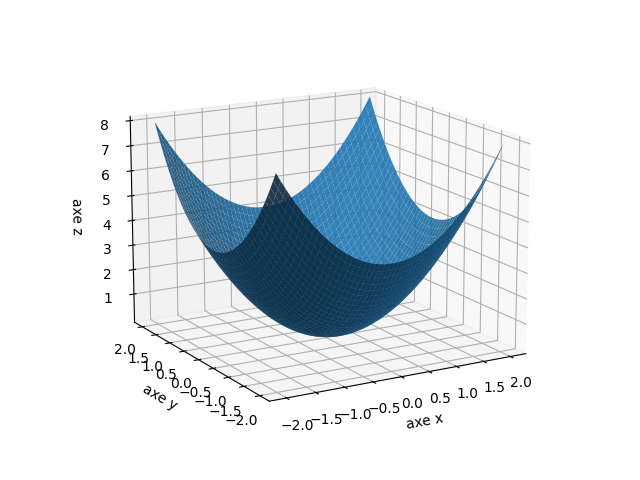
\includegraphics[scale=\myscale,scale=0.5]{figures/fonctions-extrem-1a}
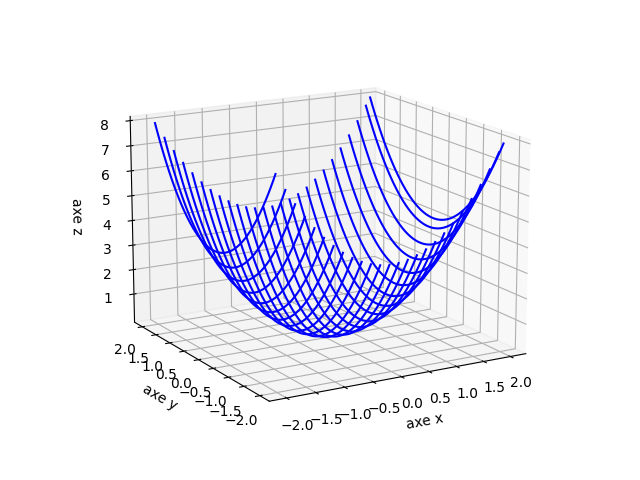
\includegraphics[scale=\myscale,scale=0.5]{figures/fonctions-extrem-1b}
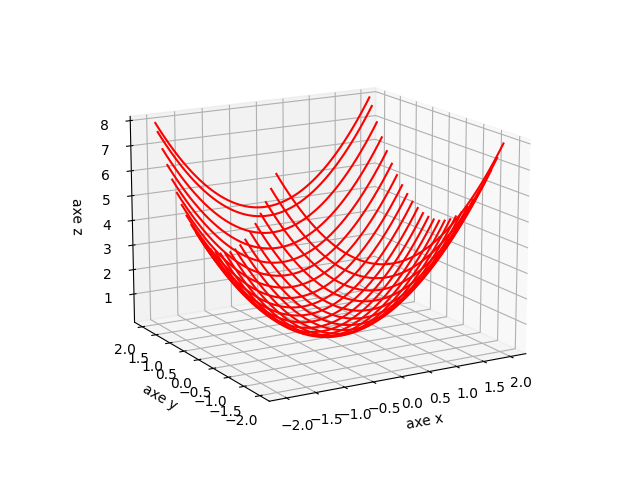
\includegraphics[scale=\myscale,scale=0.5]{figures/fonctions-extrem-1c}
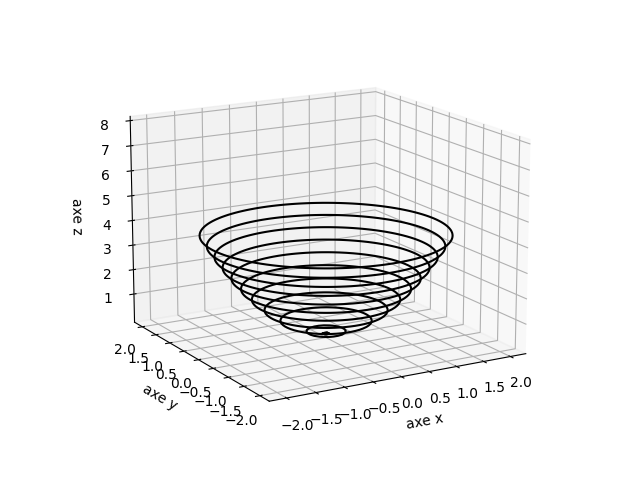
\includegraphics[scale=\myscale,scale=0.5]{figures/fonctions-extrem-1d}
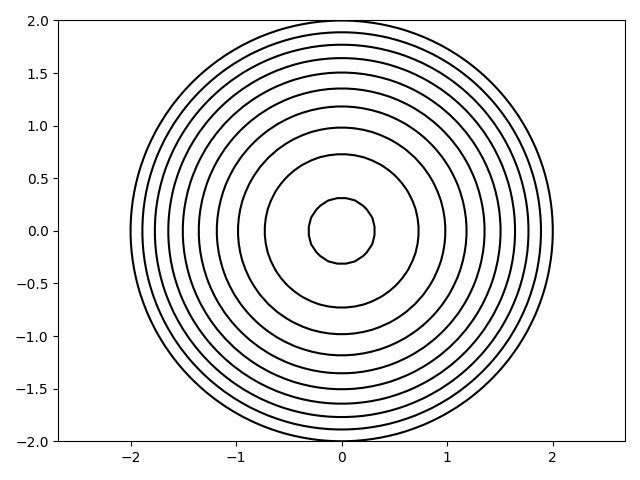
\includegraphics[scale=\myscale,scale=0.5]{figures/fonctions-extrem-1e}
\end{center}

% dessins 3d voir 'fonctions-extrem-1.py' 


	

$f(x,y) = -x^2 - y^2$. C'est un exemple de maximum local atteint en $(0,0)$.


\begin{center}
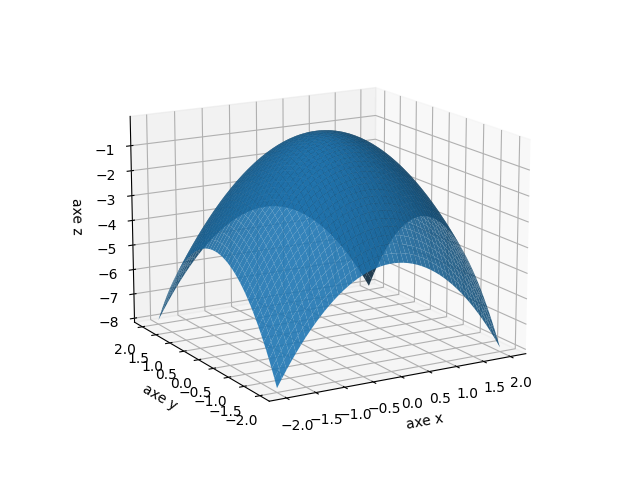
\includegraphics[scale=\myscale,scale=0.5]{figures/fonctions-extrem-2a}
\end{center}

% dessins 3d voir 'fonctions-extrem-2.py' 
	



$f(x,y) = x^2 - y^2$. C'est un exemple de point-selle en $(0,0)$.

\begin{itemize}
  \item Les tranches sont des paraboles, tournées vers le haut ou vers le bas selon la direction de la tranche.
  \item Les lignes de niveau sont des hyperboles.
  \item Le graphe est donc un \trouer{paraboloïde hyperbolique} que l'on appelle aussi la \trouer{selle de cheval}\index{point-selle}.
  \item Un autre nom pour cette surface est un \trouer{col} (en référence à un col en montagne). 
  En effet, le point $(0,0,0)$ est le point de passage le moins haut pour passer d'un versant à l'autre de la montagne. 
\end{itemize}

Ci-dessous : (a) la surface, (b) les tranches avec $x$ constant, (c) les tranches avec $y$ constant, (d) les courbes de niveau, (e) les lignes de niveau dans le plan (en pointillé les lignes de niveau négatif).
\begin{center}
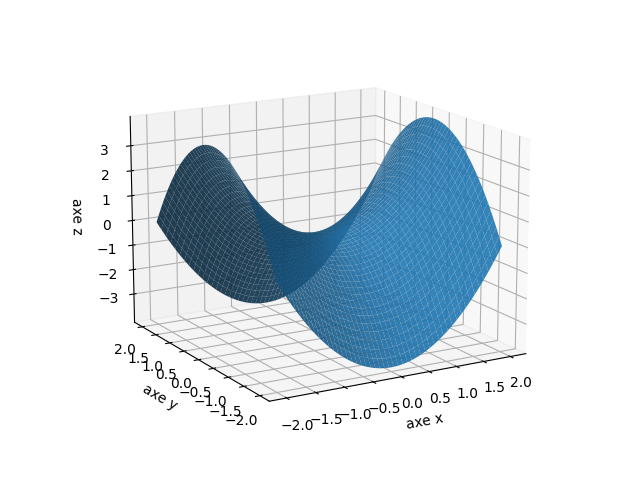
\includegraphics[scale=\myscale,scale=0.5]{figures/fonctions-extrem-3a}
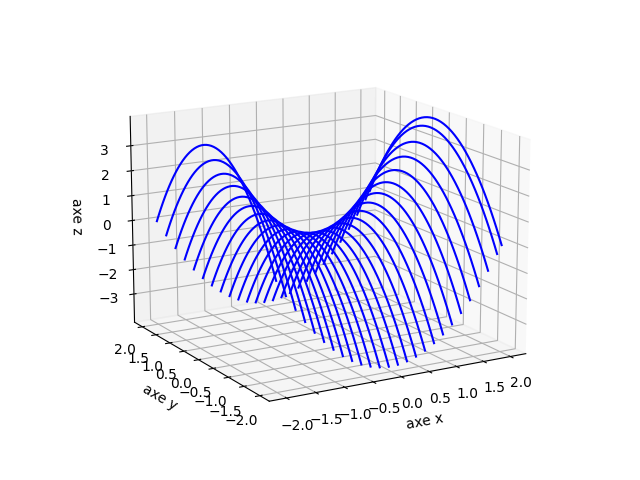
\includegraphics[scale=\myscale,scale=0.5]{figures/fonctions-extrem-3b}
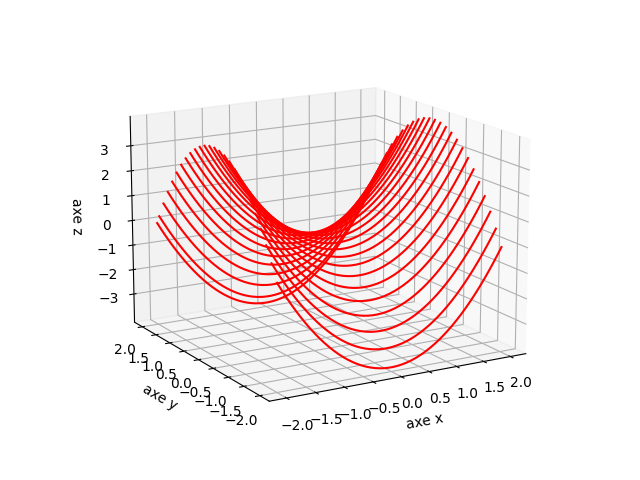
\includegraphics[scale=\myscale,scale=0.5]{figures/fonctions-extrem-3c}
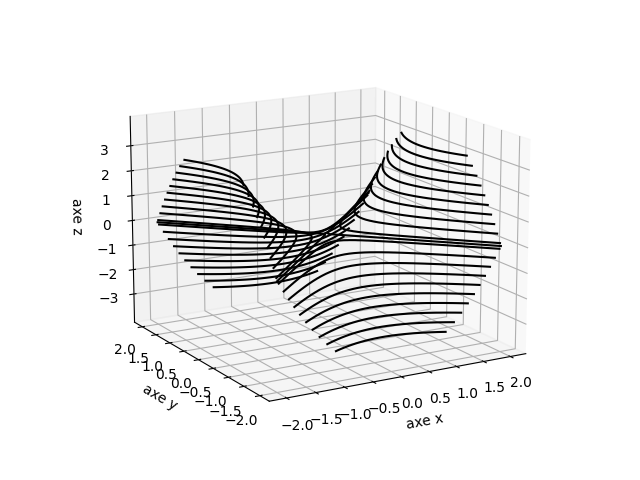
\includegraphics[scale=\myscale,scale=0.5]{figures/fonctions-extrem-3d}
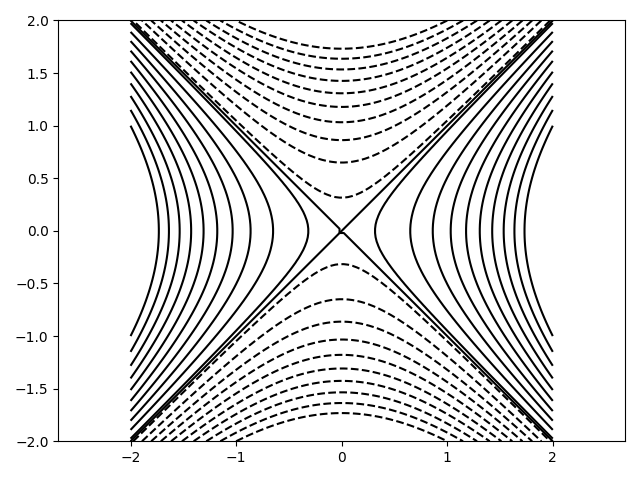
\includegraphics[scale=\myscale,scale=0.5]{figures/fonctions-extrem-3e}
\end{center}

% dessins 3d voir 'fonctions-extrem-3.py' 	






%----------------------------------------------------
\subsection{Caractérisation des minimums et maximums}

Pour une fonction $f : \Rr^2 \to \Rr$, nous utiliserons la notation de Monge, qui fournit un critère simple pour détecter un minimum ou un maximum local.
\begin{theoreme}{Critère de Monge}{}
Soit $f : \Rr^2 \to \Rr$ une fonction de classe $\mathcal{C}^2$ et soit $(x_0,y_0)$ un point critique de $f$.
 On pose 
$$
	r=\frac{\partial^2 f}{\partial x^2}(x_0,y_0)  
	\qquad 
	s=\frac{\partial^2 f}{\partial x \partial y}(x_0,y_0)
	\qquad
	t=\frac{\partial^2 f}{\partial y^2}(x_0,y_0).
$$
Alors :
\begin{itemize}
	\item si $rt-s^2>0$ et $r>0$, alors $(x_0,y_0)$ est un minimum local de $f$,
	\item si $rt-s^2>0$ et $r<0$, alors $(x_0,y_0)$ est un maximum local de $f$,
	\item si $rt-s^2<0$, alors $(x_0,y_0)$ n'est ni un minimum local ni un maximum local : c'est un point-selle,
	 \item si $rt-s^2=0$, on ne peut pas conclure directement (il faut approfondir l'étude).
\end{itemize}
\end{theoreme}

Remarque : $rt-s^2$ est le déterminant de la matrice hessienne en $(x_0,y_0)$, $H_f(x_0,y_0) = \begin{pmatrix}r&s\\s&t\end{pmatrix}$.

\begin{exemple}{}{}
Reprenons les trois exemples fondamentaux, pour vérifier notre critère.
\begin{enumerate}
	\item Soit  $f(x,y)=x^2+y^2$. Le point $(0,0$) est l'unique point critique de $f$.
On calcule 
$$r=\frac{\partial^2 f}{\partial x^2}(0,0)=2 
\qquad 
s=\frac{\partial^2 f}{\partial x \partial y}(0,0)=0
\qquad
t=\frac{\partial^2 f}{\partial y^2}(0,0)=2.$$
Ainsi, $rt-s^2 = 4$ avec $r>0$, et donc $(0,0)$ est bien un minimum local de $f$.
  \item Exercice : faire le même travail avec $f(x,y)=-x^2-y^2$. 
  \item Soit $f(x,y)=x^2-y^2$. On trouve un seul point critique : $(0,0)$. 
   On calcule $H_f(0,0) = \left(\begin{smallmatrix}2&0\\0&-2\end{smallmatrix}\right)$.
   Cette fois, $r=2$, $s=0$, $t=-2$. Ainsi, $rt-s^2 = -4 < 0$ et donc $(0,0)$ correspond bien à un point-selle.
\end{enumerate}

\end{exemple}


%----------------------------------------------------
\subsection{Autres exemples}

\begin{exemple}{}{}
Soit $f: \Rr^2 \to \Rr$ définie par $f(x,y)=x^3+y^3-3xy$.


\begin{center}
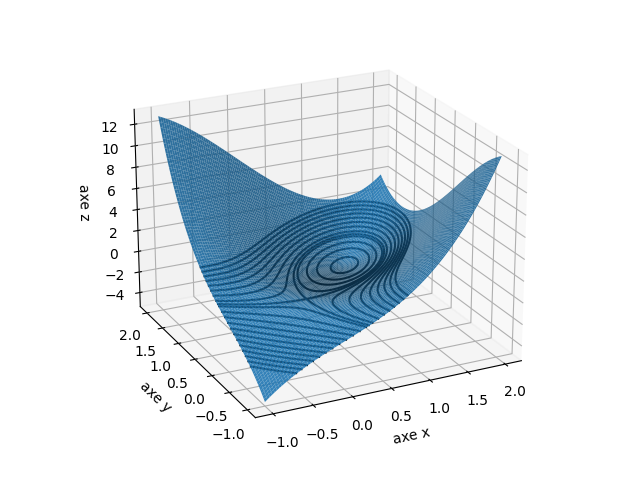
\includegraphics[scale=\myscale,scale=0.8]{figures/fonctions-extrem-4}
\end{center}

% dessins 3d voir 'fonctions-extrem-4.py' 
	

\begin{itemize}
	\item \textbf{Dérivées partielles.}
    $$\frac{\partial f}{\partial x}(x,y) = 3x^2-3y \qquad\qquad
    \frac{\partial f}{\partial y}(x,y) = 3y^2-3x$$
    	
	\item \textbf{Points critiques.}
    Ce sont les points où $\frac{\partial f}{\partial x}(x,y) = 0$ et $\frac{\partial f}{\partial y}(x,y) = 0$ en même temps. On a donc simultanément $x^2=y$ et $y^2=x$ (ce qui implique $x,y\ge0$).
    D'où $x^4 = y^2 = x$ dont les solutions positives sont $x=0$ (et alors $y=0$) et $x=1$ (et alors $y=1$). Ainsi, les points critiques sont $(0,0)$ et $(1,1)$.
	
	\item \textbf{Dérivées partielles secondes.}
    $$\frac{\partial^2 f}{\partial x^2}(x,y) = 6x
    \qquad 
    \frac{\partial^2 f}{\partial x \partial y}(x,y) = -3
    \qquad
    \frac{\partial^2 f}{\partial y^2}(x,y) = 6y$$
	
	\item \textbf{Étude en $(0,0)$.}     
    $$H_f(0,0) = \begin{pmatrix}0&-3\\-3&0\end{pmatrix}$$
    C'est-à-dire $r=0$, $s=-3$, $t=0$, donc $rt-s^2 = -9 < 0$ et donc $(0,0)$ est un point-selle.
   
	
    \item \textbf{Étude en $(1,1)$.}	
    $$H_f(1,1) = \begin{pmatrix}6&-3\\-3&6\end{pmatrix}$$
    C'est-à-dire $r=6$, $s=-3$, $t=6$, donc $rt-s^2 = 27 > 0$ avec $r>0$ et donc $(1,1)$ est un point de minimum de $f$ (c'est un minimum local et pas global).	
\end{itemize}

\end{exemple}

\bigskip	

Voici un exemple où le critère ne permet pas de conclure. Il faut terminer l'étude à la main.
\begin{exemple}{}{}
Soit $f(x,y)=2x^3-y^4-3x^2$. On trouve deux points critiques : $(0,0)$ et $(1,0)$. Par ailleurs :
$$H_f(0,0)=\begin{pmatrix}-6&0\\ 0&0\end{pmatrix}\qquad \text{ et } \qquad H_f(1,0)=\begin{pmatrix}6&0\\ 0&0\end{pmatrix}.$$
On ne peut pas conclure car le déterminant $rt-s^2$ est nul. On étudie chaque cas à la main.


\begin{center}
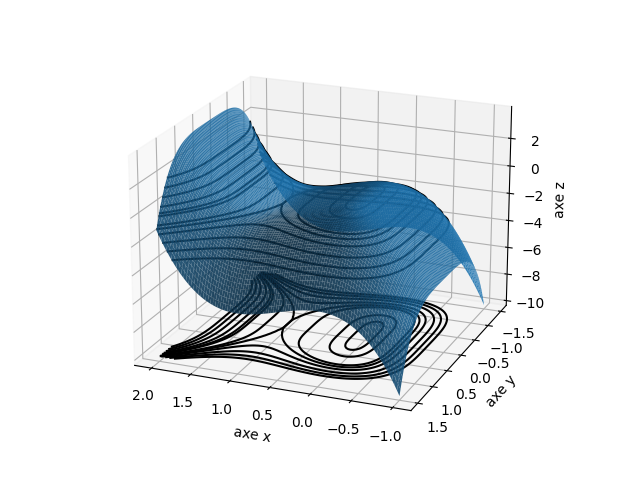
\includegraphics[scale=\myscale,scale=0.8]{figures/fonctions-extrem-5}
\end{center}

% dessins 3d voir 'fonctions-extrem-5.py' 

\begin{itemize}
	\item En $(0,0)$. 
	Écrivons $f(x,y)=x^2(2x-3)-y^4$.
	Pour $|x|\le 1$, on a $2x-3 \le0$, et donc 
	$$f(x,y)=x^2(2x-3)-y^4 \le 0.$$
	Comme $f(0,0)=0$, alors $f$ admet un maximum local au point $(0,0)$.
	
	\item  En $(1,0)$. 
	Tout d'abord, on se limite aux points de la forme $(1,y)$ (autour de $y_0=0$) :
		$$f(1,y)=-1-y^4\le -1 = f(1,0)$$
		
	Ensuite, on se limite aux points de la forme $(x,0)$ (autour de $x_0=1$, par exemple pour $x$ tel que  $|x-1|\leq 1$) : 
	$$ f(x,0)=(x-1)^2(2x+1)-1 \ge -1 = f(1,0)$$
	Donc, en $(1,0)$, ce n'est ni un minimum ni un maximum : c'est un point-selle.
	
\end{itemize}

\end{exemple}




%----------------------------------------------------
\subsection{Valeurs propres de la hessienne}

Ce paragraphe peut être omis à la première lecture.

Nous reformulons le critère précédent en termes de valeurs propres de la matrice hessienne.
Les valeurs propres de la matrice $H_f(x_0,y_0)$ sont les racines du polynôme caractéristique qui est défini par $\chi(\lambda)=\det \left( H_f(x_0,y_0)-\lambda I \right)$.

\begin{theoreme}{}{}
Soient $U$ un ouvert de $\Rr^2$, $f$ une fonction de classe $\mathcal{C}^2$ sur $U$ et $(x_0,y_0)\in U$ un point critique de $f$.
\begin{enumerate}
    \item Si $H_f(x_0,y_0)$ a ses deux valeurs propres strictement positives, alors $f$ présente un minimum en $(x_0,y_0)$.
    \item Si $H_f(x_0,y_0)$ a ses deux valeurs propres strictement négatives, alors $f$ présente un maximum en $(x_0,y_0)$.
    \item Si $H_f(x_0,y_0)$ a deux valeurs propres de signes opposés, alors $f$ ne présente pas d'extremum en $(x_0,y_0)$ : c'est un point-selle.
    \item Dans les autres cas, on ne peut rien dire (tout peut arriver).
\end{enumerate}
\end{theoreme}


%----------------------------------------------------
\paragraph{Exercices}
    \begin{enumerate}
        \item Soit $f(x,y)=\exp(-\frac 13 x^3 + x - y^2)$. Déterminer les deux points critiques de $f$ et la nature (minimum/maximum/point-selle) de chacun d'entre eux.

\begin{center}
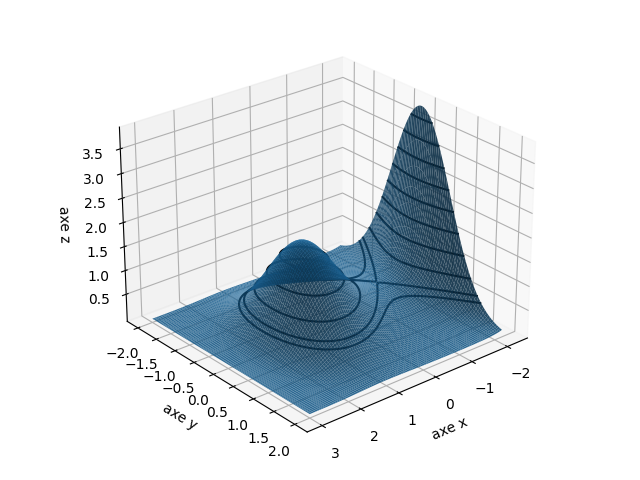
\includegraphics[scale=\myscale,scale=0.6]{figures/fonctions-extrem-7}
\end{center}

% dessins 3d voir 'fonctions-extrem-7.py' 


        \item Soit $f(x,y)=x^3-3xy^2$. Déterminer le point critique de $f$ et sa nature.
        Le graphe de $f$ s'appelle une \og{}selle de singe\fg{}.

\begin{center}
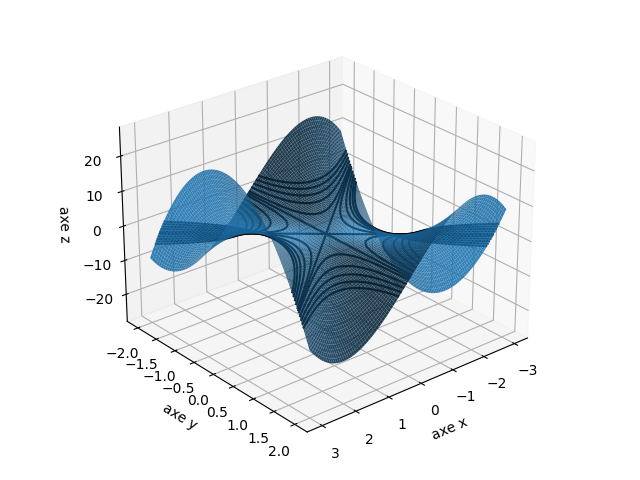
\includegraphics[scale=\myscale,scale=0.6]{figures/fonctions-extrem-6}
\end{center}

% dessins 3d voir 'fonctions-extrem-6.py' 
        
        \item Soit $f(x,y)=x^4+y^4-2x^2$. Déterminer les trois points critiques de $f$.
        Le critère de Monge permet-il de conclure ?
        Déterminer quand même la nature de chacun de ces points critiques.

%On trouve trois points critiques $(-1,0)$, $(1,0)$ et $(0,0)$. Par ailleurs,
%        $$H_f(-1,0)=H_f(1,0)=\left(\begin{array}{cc}8&0\\ 0&0\end{array}\right)\quad \mbox{ et }\quad H_f(0,0)=\left(\begin{array}{cc}-4&0\\ 0&0\end{array}\right).$$
%        On ne peut pas conclure. Or
%        $$f(x,y)=(x^2-1)^2+y^4-1\geq -1=f(\pm 1,0).$$
%        Donc $f$ admet un minimum aux points $(\pm 1,0)$. D'autre part, pour $|x|\leq 1$,
%        $$f(x,0)=x^4-2x^2=x^2(x^2-2)\leq 0=f(0,0)\quad \mbox{ et }\quad f(0,y)=y^4\geq 0=f(0,0).$$
%        Donc $(0,0)$ n'est ni un maximum ni un minimum ; c'est un point selle.


    \end{enumerate}

 


%%%%%%%%%%%%%%%%%%%%%%%%%%%%%%%%%%%%%%%%%%%%%%%%%%%%%
\section{Minimum et maximum : cas général}

Nous étendons les résultats précédents dans deux directions : tout d'abord pour les fonctions avec un nombre quelconque de variables, puis pour la recherche de minimums/maximums sur un compact.


%----------------------------------------------------
\subsection{Cas de $\Rr^n$}

Soit $n\ge2$.
Étendons les définitions au cas d'une fonction $f : U\to \Rr$, o\`u $U$ est un ouvert de $\Rr^n$.

\begin{itemize}
    \item $f$ admet un \trouer{maximum local} (resp. \trouer{minimum local}) en $x_0 \in U$ s'il existe une boule ouverte $B\subset U$ centrée en $x_0$ telle que, 
    pour tout $x \in B$, on ait $f(x) \le f(x_0)$ (resp. $f(x) \ge f(x_0)$).
        
    \item $f$ admet un \trouer{extremum local} en $x_0$ si elle y admet un maximum local ou un minimum local.
    
    \item $x_0$ est un \trouer{point critique} de $f$ si le gradient de $f$ s'annule en $x_0$, ou autrement dit si $\frac{\partial f}{\partial x_i}(x_0) = 0$ pour tout $i=1,\ldots,n$. 
      
    \item  \textbf{Proposition.} Si $f$ admet un extremum local en $x_0 \in U$ et si le gradient est défini en ce point, alors $x_0$ est un point critique de $f$.

    \item Ainsi, on cherche les extremums locaux parmi les points critiques de $f$.
\end{itemize}


    
    
%----------------------------------------------------
\subsection{Extremum sur un compact}

Pour une fonction  d'une variable $f : [a,b] \to \Rr$ continue sur un intervalle compact, on sait que $f$ est bornée et atteint ses bornes, c'est-à-dire qu'elle atteint un minimum global et atteint aussi un maximum global.  Ce minimum ou ce maximum peut être atteint au \og{}bord\fg{} du segment, c'est-à-dire en $a$ ou en $b$, ou bien à \og{}l'intérieur\fg{} $]a,b[$. 
Il faut faire attention à bien distinguer l'étude à l'intérieur et au bord. En effet, à l'intérieur, un extremum est un point critique de $f$, alors que sur le bord ce n'est plus nécessairement le cas. Garder en mémoire l'exemple $f(x) = x^2$ sur $[-1,1]$ : la dérivée s'annule en $x=0$ (minimum local et global) mais un maximum (local et global) est atteint en $x=1$ et $x=-1$ alors que la dérivée ne s'y annule pas (explication : $+1$ et $-1$ sont au bord de l'intervalle).


\myfigure{1}{
    \tikzinput{fig-extrem-07}     
}



Cette propriété se généralise aux fonctions de plusieurs variables, continues sur un ensemble compact. (Nous l'admettons.)

\begin{proposition}{}{}
Soit $f : K \rightarrow \Rr$ une fonction continue sur un ensemble compact $K \subset \Rr^n$. Alors $f$ est bornée et atteint ses extremums sur $K$.
\end{proposition}

La marche à suivre pour étudier les extremums d'une fonction différentiable sur un compact $K \subset \Rr^n$ est la suivante :
\begin{enumerate}
    \item Rechercher les points critiques dans l'intérieur de $K$.
    \item Déterminer si chacun de ces points critiques est un maximum local, un minimum local ou ni l'un ni l'autre. (Dans le cas $n=2$, on utilise les dérivées partielles secondes. Il existe des généralisations de ces formules à $n$ quelconque.)
    \item Chercher si $f$ admet des extremums sur le bord de $K$ (le critère des points critiques n'est plus valable).
    \item Comparer les minimums pour déterminer le -- ou les -- minimums globaux  ; idem pour les maximums.
\end{enumerate}

On rappelle qu'un ensemble $A \subset \Rr^n$ découpe l'espace en trois parties disjointes : son intérieur $\operatorname{Int} A$, son bord $\partial A$ (ou frontière), et son extérieur $\operatorname{Ext} A$.


\myfigure{1}{
    \tikzinput{fig-extrem-08}     
}



\begin{exemple}{}{}
Déterminons les extremums de $f$ sur $K$ où :
$$f(x,y) = x^2 - y^2 \qquad \text{ et } \qquad K = \lbrace (x,y) \in \Rr^2  \mid  x^2 + y^2 \leq 1 \rbrace.$$

\myfigure{1}{
    \tikzinput{fig-extrem-09}     
}


On procède de la manière suivante :     
\begin{enumerate}
    \item On cherche les points critiques et les extremums locaux dans $\operatorname{Int} K$.
    On trouve un seul point critique, en $(0,0)$. Mais, en $(0,0)$, $f$ a un point-selle. La fonction n'a donc pas d'extremum à l'intérieur de $K$. Mais comme $K$ est compact et $f$ est continue sur $K$, $f$ est bornée sur $K$ et atteint ses bornes sur $K$. Ce sera donc sur le bord de $K$.
    
    \item On analyse $f$ sur $\partial K$.
    Une possibilité ici est de paramétrer le bord de $K$ : c'est le cercle de rayon $1$ centré en $(0,0)$ que l'on paramètre par $(\cos t,\sin t)$, pour $t\in[0,2\pi]$. On obtient :
    $f(\cos t,\sin t)=\cos^2t-\sin^2t=\cos(2t)$. On peut alors étudier les variations de cette fonction. On obtient qu'elle est maximum, égale à $1$, lorsque $2t \equiv 0 \pmod{2\pi}$, et minimum, égale à $-1$, lorsque $2t \equiv \pi \pmod{2\pi}$. La fonction $f$ atteint donc son maximum $1$ aux points $(1,0)$ et $(-1,0)$ de $K$, et son minimum $-1$ aux points $(0,1)$ et $(0,-1)$.
\end{enumerate}

\begin{center}
  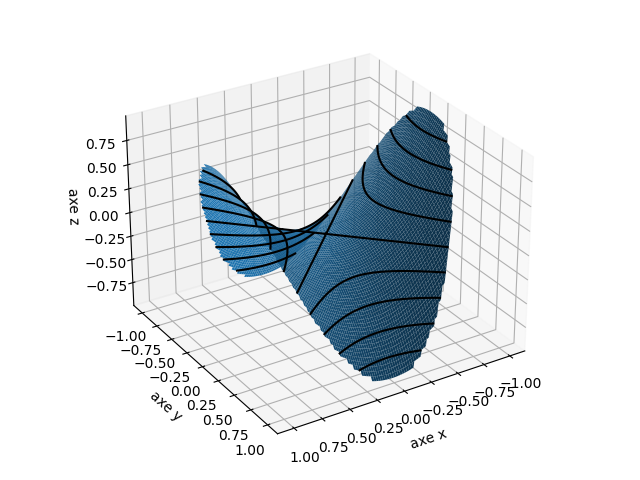
\includegraphics[scale=\myscale,scale=0.6]{figures/fonctions-extrem-8}
\end{center}

\end{exemple}



%----------------------------------------------------
\paragraph{Exercices}
    \begin{enumerate}
        \item Déterminer les extremums (locaux et globaux) de $f(x,y) = x^2+y^2$ sur $C = [-1,1] \times [-1,1]$. Même question avec $f(x,y)= xy$.

        \item Déterminer les extremums (locaux et globaux) de $f(x,y) = x^3-y^2$ sur $D = \lbrace (x,y) \in \Rr^2  \mid  x^2 + y^2 \leq 1 \rbrace$.

        \item Déterminer les extremums (locaux et globaux) de $f(x,y) = y\cos(x)$ sur $B = \Rr \times [0,1]$.
    \end{enumerate}




%%%%%%%%%%%%%%%%%%%%%%%%%%%%%%%%%%%%%%%%%%%%%%%%%%%%%%%%%%%%%%%%%%%%%

\section{Convexité}


\subsection{Définition}

\begin{definition}{}{}
	Une fonction $f : \Rr^n \to \Rr^n$ est dite convexe si pour tous $x,y \in \Rr^n$ et tout $t \in [0,1]$ on a : $$f(tx+(1-t)y) \le t f(x) + (1-t) f(y).$$ La fonction $f$ est dite strictement convexe si pour tous $x,y \in \Rr^n$ et tout $t \in ]0,1[$ on a : $$f(tx+(1-t)y) < t f(x) + (1-t) f(y).$$
\end{definition}

En d'autres termes, la droite passant par les points de coordonnées $(x,f(x))$ et $(y,f(y))$ se situe au-dessus du graphe de la fonction $f$. On peut ainsi illustrer la convexité de la fonction "valeur absolue" $x \mapsto |x|$, ici avec $x=-3$ et $y=2$ : 

\bigskip

\begin{center}
	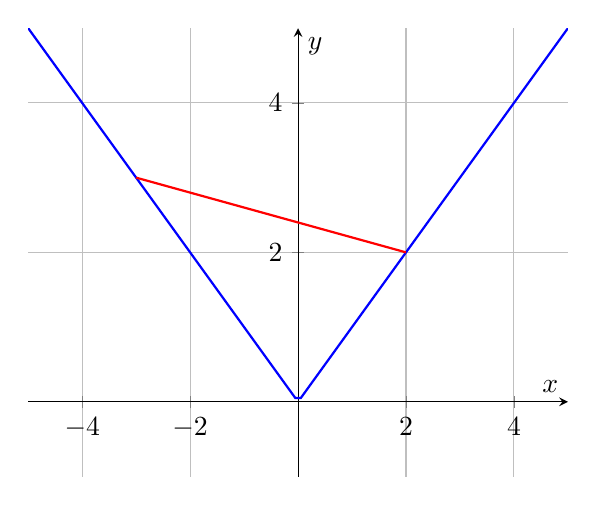
\begin{tikzpicture}
		\begin{axis}[
			axis lines = middle,
			xlabel = $x$,
			ylabel = $y$,
			xmin=-5,  
			xmax=5,
			ymin=-1, ymax=5,
			grid=major,
			]
			
			\addplot[domain=-5:5, samples=100, blue, thick] {abs(x)};
			
			% Exemple de segment pour illustrer la convexité
			\addplot[red,thick] coordinates {(-3,3)(2,2)};
			
		\end{axis}
	\end{tikzpicture}
\end{center}

De la définition de convexité on en déduit l'inégalité des pentes :

\begin{proposition}{}{}
	Soit $f : \Rr \to \Rr$ une fonction convexe et $x_1<x_2<x_3<x_4$ des réels. On a : $$\frac{f(x_2)-f(x_1)}{x_2-x_1} \le \frac{f(x_4)-f(x_3)}{x_4-x_3}.$$
\end{proposition}

Donnons une idée de la preuve : on pose $t = \frac{x_3-x_2}{x_3-x_1}$ et $s = \frac{x_4-x_3}{x_4-x_2}$, de telle sorte que $s,t \in [0,1]$ et : $$x_2 = (1-t)x_1+t x_3 \ , \ x_3 = (1-s) x_2+s x_4.$$ Par convexité de $f$ on a : $$f(x_2) \le (1-t) f(x_1)+t f(x_3) \ , \ f(x_3) \le (1-s) f(x_2)+s f(x_4).$$ En combinant ces deux inégalités on obtient : $$ts(f(x_4)-f(x_3)) \geq (1-t) (1-s) (f(x_2)-f(x_1)).$$ En remplaçant $s$ et $t$ par les expressions explicites et après simplifications on obtient le résultat voulu.

\subsection{Convexité et hessienne}

Une fonction convexe est toujours continue, mais pas forcément partout différentiable : pour un contre-exemple, il suffit de considérer la fonction "valeur absolue" $x \mapsto |x|$, qui n'est pas dérivable en $0$.

\bigskip

\begin{proposition}{}{}
	Une fonction $f : \Rr \to \Rr$ de classe $\mathcal{C}^2$ est convexe si et seulement si sa dérivée seconde vérifie $f'' \geq 0$.
\end{proposition}

\begin{proof}
	On suppose que $f$ est convexe et de classe $\mathcal{C}^2$. On veut montrer que la dérivée seconde $f''$ est à valeurs positives. Pour ce faire, on va montrer que la dérivée première $f'$ est une fonction croissante. Soient $x<y$ deux réels et $h>0$ petit. L'inégalité des pentes appliquée à $x,x+h,y,y+h$ s'écrit : $$\frac{f(x+h)-f(x)}{h} \le \frac{f(y+h)-f(y)}{h}.$$ En faisant tendre $h \to 0$, on obtient l'inégalité entre dérivées à droite $f'(x) \le f'(y)$ donc $f'$ est bien croissante.
	
	\bigskip
	
	Réciproquement, soit $f : \Rr \to \Rr$ de classe $\mathcal{C}^2$ vérifiant $f'' \ge 0$. Soient $x \le y \in \Rr$ et $t \in [0,1]$. On pose $z = (1-t) x + t y$, de telle sorte que $x \le z \le y$. Le théorème des accroissements finis donne l'existence de $a \in [x,z]$ et de $b \in [z,y]$ tels que $f'(a) = \frac{f(z)-f(x)}{z-x}$ et $f'(b) = \frac{f(y)-f(z)}{y-z}$. Comme $a \le b$, on a $f'(a) \le f'(b)$, donc $$(f(z)-f(x))(y-z) \le (f(y)-f(z))(z-x).$$ En remarquant que $t = \frac{z-x}{y-x}$, la dernière inégalité se transforme facilement en $f(z) \le (1-t) f(x) + t f(y)$, donc $f$ est bien convexe.
\end{proof}

On souhaite généraliser cette propriété aux fonctions à plusieurs variables. Le problème qui se présente immédiatement est que la notion de dérivée seconde se généralise en matrice hessienne.

\begin{definition}{}{}
	Une matrice symétrique $H$ est dite positive, et on note $H \ge 0$, si toutes ses valeurs propres sont positives, ou de façon équivalente si on a ${}^TX H X \ge 0$ pour tout vecteur colonne $X$.
	Une matrice symétrique $H$ est dite définie positive, et on note $H > 0$, si toutes ses valeurs propres sont strictement positives, ou de façon équivalente si on a ${}^TX H X > 0$ pour tout vecteur colonne $X \neq 0$. 
\end{definition}

On rappelle qu'une matrice symétrique réelle est diagonalisable dans $\Rr$ : elle possède une base de vecteurs propres associés à des valeurs propres qui sont toutes réelles.

\bigskip

Le lien entre convexité et dérivée seconde s'énonce alors comme suit : 
\begin{proposition}{}{}
	Soit $f : \Rr^n \to \Rr$ une fonction de classe $\mathcal{C}^2$. La fonction $f$ est convexe si et seulement si pour tout $x \in \Rr^n$ on a $H_f(x) \ge 0$.
\end{proposition}

On peut illustrer cette propriété dans le cas d'un polynôme de degré $2$ : 

\begin{exemple}{}{}
	On considère la fonction $f(x,y) = a x^2 + b xy + c y^2$. La hessienne de $f$ est constante, c'est la matrice $H = \begin{pmatrix} 2a & b \\ b & 2c \end{pmatrix}$. Les valeurs propres sont obtenues par recherche des racines du polynôme caractéristique, ce sont $$\lambda_1 = (a+c) - \sqrt{(a-c)^2+b^2} \ , \ \lambda_2 = (a+c) + \sqrt{(a-c)^2+b^2}.$$ Elles sont toutes les deux positives si et seulement si $a+c \ge 0$ et $(a+c)^2 \ge (a-c)^2+b^2$, c'est-à-dire $b^2 \le 4 ac$. Ainsi $f$ est convexe si et seulement si la trace et le déterminant de $H$ sont positifs.
\end{exemple}

Une autre famille d'exemples se rencontre assez souvent en science des données : 

\begin{exemple}{}{}
	Soit $\phi : \Rr \to \Rr$ une fonction convexe. On définit la fonction $f : \Rr^n \to \Rr$ par $f(x_1,\ldots,x_n) = \sum_{i=1}^n \phi(x_i)$. La hessienne de $f$ est simple à calculer, on a : $$H_f(x_1,\ldots,x_n) = \textrm{Diag}(\phi''(x_1),\ldots,\phi''(x_n)).$$ Les valeurs propres de la matrice hessienne sont simplement les valeurs $\phi''(x_i)$, pour $1 \le i \le n$, et sont positives par convexité de $\phi$. Ainsi la fonction $f$ est convexe.
\end{exemple}


La proposition suivante permet de relier stricte convexité avec la hessienne : 
\begin{proposition}{}{}
	Soit $f : \Rr^n \to \Rr$ une fonction de classe $\mathcal{C}^2$. On suppose que pour tout $x \in \Rr^n$ on a $H_f(x) > 0$. Alors la fonction $f$ est strictement convexe.
\end{proposition}

Remarquons que la réciproque n'est pas vraie : la fonction $f : x \mapsto x^2$ est strictement convexe mais on a $f''(0)=0$.

\subsection{Convexité et optimisation}

\begin{proposition}{}{}
	Soit $f : \Rr^n \to \Rr$ une fonction strictement convexe. Alors $f$ possède au plus un minimum local.
\end{proposition}

\begin{proof}
	On donne une idée preuve pour une fonction d'une seule variable. Supposons qu'il existe deux minimums locaux en $x_1$ et en $x_2$, avec $x_1<x_2$. On a, pour tout $t \in ]0,1[$, $f((1-t)x_1+tx_2) < (1-t) f(x_1) + t f(x_2)$. Par définition d'un minimum local, on a pour $t$ suffisamment petit, $f(x_1) \le f((1-t)x_1+tx_2)$, d'où on déduit que $f(x_2) \ge f(x_1)$. En considérant le fait que $x_2$ est un minimum local, on obtient de même que $f(x_2) \ge f(x_1)$, et donc $f(x_1)=f(x_2)$. Ainsi on a donc $f((1-t)x_1+tx_2) < f(x_1)$ pour tout $t \in ]0,1[$, ce qui, en prenant $t$ proche de $0$, contredit le fait que $x_1$ est un minimum local.
\end{proof}

Une fonction strictement convexe peut ne pas posséder de minimum local : la fonction identité $x \mapsto x$ est un contre-exemple. Mais sous certaines conditions (par exemple, si $f$ est définie sur un compact $K \subset \Rr^n$), on peut s'assurer de l'existence, donc de l'unicité, d'un minimum local, qui est alors un minimum global pour la fonction.

\bigskip

Cette propriété des fonctions strictement convexes en font des objets agréables à étudier en optimisation : un algorithme convergeant dans le cas général vers un minimum local convergerait dans ce cadre vers l'unique minimum global, ce qui est une réponse bien plus satisfaisante au problème initial.


%%%%%%%%%%%%%%%%%%%%%%%%%%%%%%%%%%%%%%%%%%%%%%%%%%%%%%%%%%%%%%%%%%%%%
\section{Méthodes d'optimisation}

Nous allons d'une part découvrir des méthodes de résolution  des problèmes d'optimisation : quelle droite approche au mieux un nuage de points, et d'autre part étudier comment améliorer le choix du pas $\delta$.



%--------------------------------------------------------------------
\subsection{Faire varier le pas}

On se concentre d'abord sur le choix du  \trouer{pas}\index{descente de gradient!pas} $\delta$ (\emph{learning rate}).

Rappelons tout d'abord que lorsque l'on se rapproche d'un point minimum, le gradient tend vers $0$. Le vecteur $\delta \grad f(P_k)$ tend donc vers $0$ à l'approche du minimum, même si $\delta$ reste constant.

Cependant, il faut choisir $\delta$ ni trop grand, ni trop petit : $\delta$ ne doit pas être trop grand car sinon les points $P_k$ vont osciller autour du minimum, mais si $\delta$ est trop petit alors les points $P_k$ ne s'approcheront du minimum qu'au bout d'un temps très long. Une solution est de faire varier $\delta$. Pour les premières itérations, on choisit un $\delta_k$ assez grand, puis de plus en plus petit au fil des itérations.

Voici différentes formules possibles, à chaque fois $\delta_0$ est le pas initial (par exemple $\delta_0=0.1$ ou $\delta_0=0.01$).

\textbf{Décroissance linéaire.}
$$\delta_k = \frac{\delta_0}{k+1}.$$

\textbf{Décroissance quadratique.}
$$\delta_k = \frac{\delta_0}{(k+1)^2}.$$

\textbf{Décroissance exponentielle.}
$$\delta_k = \delta_0 e^{-\beta k}$$
où $\beta$ est une constante positive.


\textbf{Décroissance linéaire utilisée par keras}
$$\delta_k = \frac{\delta_0}{\alpha k+1}$$
où $\alpha\ge0$ est une constante (appelée \emph{decay}).
Si $\alpha=0$ alors $\delta_k$ est constant (et vaut $\delta_0$).
L'usage courant est d'utiliser des valeurs de $\alpha$ entre $10^{-4}$ et $10^{-6}$.


Terminons par rappeler que le bon choix d'un $\delta$ ou des $\delta_k$ n'a rien d'évident, il s'obtient soit par test à la main, soit par des expérimentations automatiques, mais à chaque fois il doit être adapté à la situation.



%--------------------------------------------------------------------
\subsection{Régression linéaire $y=ax+b$}

\index{regression lineaire@régression linéaire}

On considère un ensemble de $N$ points $A_i = (x_i,y_i)$, $i=1,\ldots,N$.
L'objectif est de trouver l'équation $y=ax+b$ de la droite qui approche au mieux tous ces points. Précisons ce que veut dire \og{}approcher au mieux\fg{} : il s'agit de minimiser la somme des carrés des distances verticales entre les points et la droite.


\myfigure{1}{
	\tikzinput{fig-regression-01}
}

La formule qui donne l'erreur est :
$$E(a,b) = \sum_{i=1}^{N}\big(y_i - (ax_i+b)\big)^2,$$
autrement dit 
$$E(a,b) = \big(y_1 - (ax_1+b)\big)^2 + \cdots + \big(y_N - (ax_N+b)\big)^2.$$

Remarquons que l'on a toujours $E(a,b)\ge0$. Si par exemple tous les points sont alignés, alors on peut trouver $a$ et $b$ tels que $E(a,b)=0$. Quand ce n'est pas le cas, on cherche $a$ et $b$ qui rendent $E(a,b)$ le plus petit possible.
Il s'agit donc bien ici de minimiser une fonction de deux variables (les variables sont $a$ et $b$).

Nous allons appliquer la méthode de la descente de gradient à la fonction $E(a,b)$. Pour cela nous aurons besoin de calculer son gradient :
$$\grad E(a,b) 
= \left(\frac{\partial E}{\partial a}(a,b), \frac{\partial E}{\partial b}(a,b)\right)
= \left(
\sum_{i=1}^{N} -2x_i\big(y_i - (ax_i+b)\big),  
\sum_{i=1}^{N} -2\big(y_i - (ax_i+b)\big)
\right).$$


\begin{exemple}{}{}
	Prenons d'abord l'exemple de trois points $A_1 = (0,3)$, $A_2 = (2,4)$ et $A_3 = (6,6)$ qui sont alignés. 
	
	\myfigure{1}{
		\tikzinput{fig-regression-02}
	}
	
	La fonction $E(a,b)$ s'écrit :
	$$E(a,b) = (3-b)^2 + (4-(2a+b))^2 + (6-(6a+b))^2.$$
	Partons arbitrairement de $(a_0,b_0) = (0,1)$ (qui correspond à la droite horizontale d'équation $y=1$).
	Voici les valeurs successives $(a_k,b_k)$ obtenues par la méthode de descente de gradient pour un pas $\delta = 0.02$.
	
	$$
	\begin{array}{c|c|c|c}
		k & (a_k,b_k) & \grad E(a_k,b_k) & E(a_k,b_k) \\ \hline
		0 & (0, 1) & (-72 -20) &  38 \\
		1 & (1.44, 1.4) & (49.60, 5.44) &  18.96 \\
		2 & (0.44, 1.29) & (-31.50, -11.08) & 10.28 \\
		3 & (1.07, 1.51) & (22.44, 0.32) &  6.24 \\
		4 & (0.62, 1.50) & (-13.57, -6.89) &  4.27 \\
		5 & (0.90, 1.64) & (10.35, -1.72) &  3.24 \\
	\end{array}
	$$
	
	\smallskip
	
	Au bout de $100$ itérations, on obtient $a_{100} \simeq 0.501$ et $b_{100} \simeq 2.99$ (avec un gradient et une erreur presque nuls). C'est bien la droite $y = \frac12x+3$ qui passe par les trois points.
	
	
	Sur la figure de gauche ci-dessous, sont dessinés, dans le plan de coordonnées $(a,b)$, les premiers points $(a_k,b_k)$ qui convergent (lentement et en oscillant) vers $(\frac12,3)$\couleurnb{ (point bleu)}{}. Sur la figure de droite sont tracées, dans le plan de coordonnées $(x,y)$, les droites d'équation $y = a_kx+b_k$ pour les premières valeurs de $k$. 
	Il est beaucoup plus difficile d'appréhender la convergence des droites (vers la droite d'équation $y=\frac12x+3$\couleurnb{ en bleu}{}) que celle des points de la figure de gauche.
	
	\begin{center}
		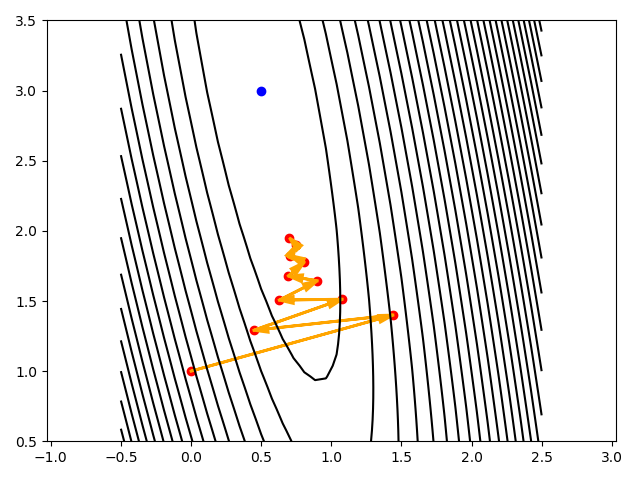
\includegraphics[scale=\myscale,scale=0.5]{figures/regression-01}
		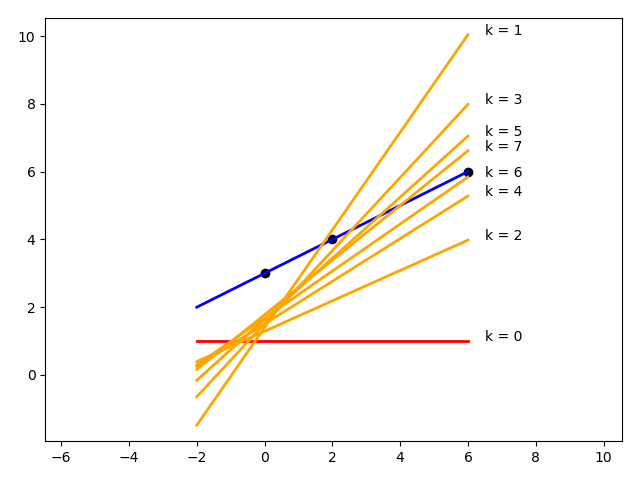
\includegraphics[scale=\myscale,scale=0.5]{figures/regression-02}
	\end{center}
\end{exemple}

\begin{exemple}{}{}
	\`A partir des données des $5$ points suivants, quelle ordonnée peut-on extrapoler pour le point d'abscisse $x=6$ ?
	
	$$A_1 = (4,1),\quad A_2 = (7,3),\quad A_3 = (8,3),\quad A_4 = (10,6),\quad A_5 = (12,7).$$
	\myfigure{0.5}{
		\tikzinput{fig-regression-03}
	}
	
	Ces $5$ points sont à peu près alignés. On calcule la meilleure droite de régression linéaire par la descente de gradient. Cela revient par exemple à minimiser la fonction $E(a,b)$ présentée ci-dessus, mais actualisée avec nos données. 
	On fixe un pas $\delta = 0.001$.
	On ne choisit pas le point initial $(a_0,b_0)$ au hasard. Plus on part d'un point proche de la solution, plus la suite convergera rapidement. On trace la droite qui passe par le premier point $A_1$ et le dernier point $A_5$. Cette droite a pour équation $y=\frac34 x -2$ et est déjà une droite qui approche assez bien les $5$ points. Prenons cette droite comme point de départ, c'est-à-dire posons $(a_0,b_0) = (\frac34,-2)$.
	La descente de gradient conduit au bout de $1000$ itérations à $a\simeq 0.78$ et $b\simeq -2.46$, pour l'équation de la droite de régression linéaire.
	
	Sur le dessin ci-dessous sont tracées la droite initiale qui passe par les points $A_1$ et $A_5$ \couleurnb{(en rouge) }{}et la droite de régression linéaire\couleurnb{ (en bleu)}{}.
	
	\myfigure{0.5}{
		\tikzinput{fig-regression-04}
	}
	
	N'oublions pas de répondre à la question initiale. Selon notre modèle linéaire, pour $x=6$, on doit avoir $y=ax+b \simeq 2.22$ (le point $B$ de la figure ci-dessus).
\end{exemple}

Remarque : il existe une formule directe pour calculer exactement les coefficients $a$ et $b$ de la droite de régression linéaire, mais ce n'est pas l'esprit de ce cours.


%--------------------------------------------------------------------
%\subsection{Régression linéaire et neurone}
%
%Quel est le lien entre la régression linéaire et un neurone ?
%En fait, le neurone suivant a pour fonction associée $F(x) = ax+b$.
%
%\myfigure{1}{
%	\tikzinput{fig-regression-05}
%}
%
%Reformulons le problème de la régression linéaire ainsi : soit des données $(x_i,y_i)$, $i=1,\ldots,N$. Il s'agit de trouver pour le type de neurone choisi les coefficients $a$ et $b$, tels que la fonction $F$ associée au neurone réalise au mieux ces données, c'est-à-dire 
%$$F(x_i) \simeq y_i.$$
%
%Vocabulaire :
%\begin{itemize}
%	\item Chaque $x_i$ est une  \trouer{entrée},
%	\item $y_i$ est la  \trouer{sortie attendue} pour l'entrée $x_i$,
%	\item $F(x_i)$ est la  \trouer{sortie produite},
%	\item $E_i = (y_i - F(x_i))^2$ est l'erreur pour l'entrée $x_i$,
%	\item  \trouer{L'erreur totale} est $$E = \sum_{i=1}^N E_i =  \sum_{i=1}^N(y_i - F(x_i))^2.$$
%	\item Vu que $F(x)=ax+b$, on retrouve bien pour $E$ la forme de la fonction présentée précédemment.
%\end{itemize}


%--------------------------------------------------------------------
%\subsection{Régression linéaire $z=ax+by+c$}
%
%Le neurone suivant a pour fonction $F(x,y) = ax+by+c$.
%Le problème de la régression linéaire pour un tel neurones et des données $(x_i,y_i,z_i)$,  $i=1,\ldots,N$, consiste à trouver des poids $(a,b,c)$ tels que $F(x_i,y_i) \simeq z_i$.
%
%\myfigure{1}{
%	\tikzinput{fig-regression-06}
%}
%
%En terme géométrique, il s'agit de trouver un plan d'équation $z=ax+by+c$ qui approche au mieux des points donnés de l'espace $(x_i,y_i,z_i)$. 
%
%\myfigure{0.8}{
%	\tikzinput{fig-regression-07}
%}
%
%
%La méthode est la même que précédemment, il s'agit de minimiser la fonction erreur de trois variables :
%$$E(a,b,c) = \sum_{i=1}^N \big(z_i - (ax_i+by_i+c)\big)^2.$$
%On aura besoin de calculer le gradient de $E$ :
%$$\grad E(a,b,c) 
%= \left(\frac{\partial E}{\partial a}(a,b,c), \frac{\partial E}{\partial b}(a,b,c), \frac{\partial E}{\partial c}(a,b,c)\right).$$
%On a : 
%{\small
%	$$\grad E(a,b,c) 
%	= \left(
%	\sum_{i=1}^{N} -2x_i\big(z_i - (ax_i+by_i+c)\big),  
%	\sum_{i=1}^{N} -2y_i\big(z_i - (ax_i+by_i+c)\big), 
%	\sum_{i=1}^{N} -2\big(z_i - (ax_i+by_i+c)\big)
%	\right).$$
%}
%
%\begin{exemple}
%	Voici un exemple avec trois points $A_1=(0,0,3)$, $A_2=(1,0,4)$ et $A_3=(0,1,5)$.
%	Trois points appartiennent nécessairement à un plan. Nous cherchons donc l'équation $z=ax+by+c$ de ce plan.
%	La fonction d'erreur est :
%	$$E(a,b,c) = 
%	\big(3 - c\big)^2
%	+ \big(4 - (4a+c)\big)^2
%	+ \big(5 - (b+c)\big)^2.$$
%	La descente de gradient appliquée à cette fonction avec un pas $\delta = 0.2$ et
%	des valeurs initiales $(a_0,b_0,c_0)=(0,0,0)$ conduit à une suite $(a_k,b_k,c_k)$ qui tend vers $(a,b,c) = (1,2,3)$. Le plan recherché est donc $z=x+2y+3$.
%\end{exemple}
%
%
%\begin{exemple}
%	Voici un jeu de cinq données
%	$$(1,0,0),\quad (0,1,5),\quad (2,1,1),\quad (1,2,0),\quad (2,2,3).$$
%	\`A partir des données des $5$ points ci-dessus, quelle est la troisième coordonnée $z$ du point tel que $x=1$ et $y=1$ du plan qui les extrapole ?
%	
%	%Quelle sortie $z$ peut être extrapolée, suivant un modèle linéaire, pour une entrée $(x,y) = (1,1)$ ?
%	
%	Les points ne sont pas coplanaires. On cherche donc le plan qui approche au mieux ces cinq points.
%	La descente de gradient pour la fonction $E(a,b,c)$ avec $\delta=0.01$ et un point initial $(a_0,b_0,c_0)=(0,0,0)$ conduit au plan $z=ax+by+c$ avec $a\simeq-1.22$, $b\simeq0.77$, $c\simeq 2.33$ pour lesquels la valeur de $E$ est minimale avec $E(a,b,c) \simeq 14.44$.
%	
%	Pour $(x,y) = (1,1)$, la sortie produite par le modèle linéaire est $z = ax+by+c \simeq 1.88$.
%\end{exemple}



%%%%%%%%%%%%%%%%%%%%%%%%%%%%%%%%%%%%%%%%%%%%%%%%%%%%%%%%%%%%%%%%%%%%%
\section{Descente de gradient stochastique}

\index{descente de gradient!stochastique}

La descente de gradient stochastique (abrégée en \emph{sgd}) est une façon d'optimiser les calculs
de la descente de gradient pour une fonction d'erreur associée à une grande série de données.
Au lieu de calculer un gradient (compliqué) et un nouveau point pour l'ensemble des données, on calcule un gradient (simple) et un nouveau point par donnée, il faut répéter ce processus pour chaque donnée.

%--------------------------------------------------------------------
\subsection{Petits pas à petits pas}

Revenons à l'objectif visé par la régression linéaire.

On considère des données $(X_i,y_i)$, $i=1,\ldots,N$ où $X_i \in \Rr^\ell$ et $y_i \in \Rr$.
Ces données proviennent d'observations ou d'expérimentations. 

Il s'agit de trouver une fonction $F : \Rr^\ell \to \Rr $ qui modélise au mieux ces données, c'est-à-dire telle que 
$$F(X_i) \simeq y_i.$$
Pour  \trouer{l'entrée} $X_i$, la valeur $y_i$ est la  \trouer{sortie attendue}, alors que $F(X_i)$ est la  \trouer{sortie produite} par notre modèle. 

Pour mesurer la pertinence de la fonction $F$, on introduit la fonction d' \trouer{erreur totale} qui mesure l'écart entre la sortie attendue et la sortie produite :
$$E = \sum_{i=1}^N E_i =  \sum_{i=1}^N(y_i - F(X_i))^2.$$
Cette erreur totale est une somme d' \trouer{erreurs locales} :
$$E_i =  (y_i - F(X_i))^2.$$

Le but du problème est de déterminer la fonction $F$ qui minimise l'erreur $E$.
Par exemple, dans le cas de la régression linéaire, il fallait trouver les paramètres $a$ et $b$ pour définir $F(x) = ax+b$, ou bien, pour deux variables, les paramètres $a$, $b$, $c$ pour définir $F(x,y) = ax+by+c$.

Considérons une fonction erreur $E : \Rr^n \to \Rr$ qui dépend de $n$ paramètres $a_1,\ldots,a_n$ (qui définissent l'expression de la fonction $F$). 

\bigskip

\textbf{Descente de gradient classique.}
Pour minimiser l'erreur et déterminer les meilleurs paramètres, on peut appliquer la méthode du gradient classique.

On part d'un point $P_0 = (a_1,\ldots,a_n) \in \Rr^n$, puis on applique la formule de récurrence :
$$P_{k+1} = P_k - \delta \grad E (P_k).$$


Pour appliquer cette formule, il faut calculer des gradients $\grad E(P_k)$, or
$$\grad E(P_k) = \sum_{i=1}^N \grad E_i(P_k).$$

Il faut donc calculer une somme de $N$ termes à chaque itération, ce qui pose des problèmes d'efficacité pour de grandes valeurs de $N$.

\bigskip

\textbf{Descente de gradient stochastique.}

Pour diminuer la quantité de calculs, l'idée est de considérer à chaque itération un seul gradient $E_i$ à la place de $E$. C'est-à-dire : 
$$P_{k+1} = P_k - \delta \grad E_i (P_k)$$
pour \emph{une seule erreur $E_i$} (correspondant à la donnée numéro $i$).
L'itération suivante se basera sur l'erreur $E_{i+1}$.


Quel est l'intérêt de cette méthode ? 
Dans la méthode de gradient classique, on calcule à chaque itération un \og{}gros\fg{} gradient (associé à la totalité des $N$ données) qui nous rapproche d'un grand pas vers le minimum.
Ici on calcule $N$ \og{}petits\fg{} gradients qui nous rapprochent du minimum.% par $N$ petits pas. 


\myfigure{0.9}{
	\tikzinput{fig-stochastique-01}
}



Voici les premières itérations de cet algorithme.
\begin{itemize}
	\item On part d'un point $P_0$.
	
	\item On calcule $P_1 = P_0 - \delta \grad E_1 (P_0)$. C'est la formule du gradient, mais seulement pour l'erreur locale $E_1$ (juste à partir de la première donnée $(X_1,y_1)$).
	
	\item On calcule $P_2 = P_1 - \delta \grad E_2 (P_1)$. C'est la formule du gradient, mais seulement pour l'erreur locale $E_2$.
	
	\item On itère encore et encore.
	
	\item On calcule $P_{N} = P_{N-1} - \delta \grad E_N (P_{N-1})$. C'est la formule du gradient, mais seulement pour l'erreur locale $E_N$. À ce stade de l'algorithme, nous avons tenu compte de toutes les données. 
	
	\item On calcule $P_{N+1} = P_{N} - \delta \grad E_1 (P_{N})$. On recommence pour $P_N$ et l'erreur locale $E_1$.
	
	\item Etc. On s'arrête au bout d'un nombre d'étapes fixé à l'avance ou lorsque l'on est suffisamment proche du minimum.   
\end{itemize}


\begin{exemple}{}{}
	On considère les quatre points :
	$$A_1=(2,0), \quad A_2=(0,2), \quad A_3=(4, 6), \quad A_4=(1,0).$$ 
	Comme ces points ne sont clairement pas alignés, on cherche un modèle pour les placer au mieux sur une parabole.
	
	\myfigure{1}{
		\tikzinput{fig-stochastique-03}
	}
	
	On va ici chercher des coefficients $a$ et $b$ tels que les points soient proches de la parabole d'équation $y=x^2+ax+b$.
	On note donc $F(x) = x^2+ax+b$ et on souhaite $F(x_i) \simeq y_i$ pour les points $A_i = (x_i,y_i)$, $i=1,\ldots,4$.
	
	Les fonctions d'erreurs locales sont :
	$$E_i(a,b) = \big(y_i - (x_i^2+ax_i+b)\big)^2.$$
	
	La fonction d'erreur globale est :
	$$E(a,b) = E_1(a,b)+E_2(a,b)+E_3(a,b)+E_4(a,b).$$
	
	%Voici le schéma de principe de la descente de gradient stochastique (à droite) par rapport à la descente de gradient classique (à gauche).
	%
	%[[schéma]]
	
	Voici les premières itérations pour chacune des méthodes, la descente de gradient classique (à gauche), la descente de gradient stochastique (à droite) toutes les deux en partant du point $(a_0,b_0)=(1,1)$ et avec $\delta = 0.01$.
	
	\begin{center}
		\begin{minipage}{0.35\textwidth}
			\begin{center}
				{\bf Descente de gradient}
				$$
				\begin{array}{c|c|c}
					k & (a_k,b_k) & E(a_k,b_k) \\ \hline
					0 & (1, 1) & 284 \\
					&&\\
					&&\\
					&&\\
					1 & (-0.54,0.52) & 84.87 \\
					&&\\
					&&\\
					&&\\
					2 & (-1.36, 0.29) & 28.68 \\
				\end{array}
				$$
			\end{center}
		\end{minipage}
		\begin{minipage}{0.45\textwidth}
			\begin{center}
				{\bf Descente de gradient stochastique}
				$$
				\begin{array}{c|c|c}
					k & (a_k',b_k') & E(a_k',b_k') \\ \hline
					0 & (1, 1) & 284 \\
					1 & (0.72, 0.86) & 236.43 \\
					2 & (0.72, 0.88) & 237.41 \\
					3 & (-0.38, 0.60) & 100.74 \\
					4 & (-0.40, 0.58) & 97.917 \\
					5 & (-0.55, 0.50) & 83.245 \\
					6 & (-0.55, 0.53) & 83.913 \\
					7 & (-1.22, 0.37) & 36.48 \\
					8 & (-1.22, 0.36) & 36.29 \\
				\end{array}
				$$
			\end{center}
		\end{minipage}
	\end{center}
	
	Au bout de $200$ itérations la descente de gradient classique conduit à $(a_{200},b_{200}) \simeq (-2.9981, 1.9948)$ (chaque donnée a été utilisée $200$ fois).
	
	Cela correspond à $800$ itérations de la descente de gradient stochastique (chacune des $4$ données a été utilisée $200$ fois) cela conduit à 
	$(a_{800}',b_{800}') \simeq (-2.9984, 1.9954)$. 
	La limite cherchée étant $(a,b) = (-3,2)$, avec $E(a,b)=0$, les deux méthodes convergent à la même vitesse. Chaque calcul de gradient de la méthode stochastique est très simple, mais il faut plus d'itérations.
	
	
	Voici les points des premières itérations correspondant au tableau ci-dessus.
	\begin{center}
		\begin{minipage}{0.48\textwidth}
			\begin{center}
				{\bf Descente de gradient classique}
				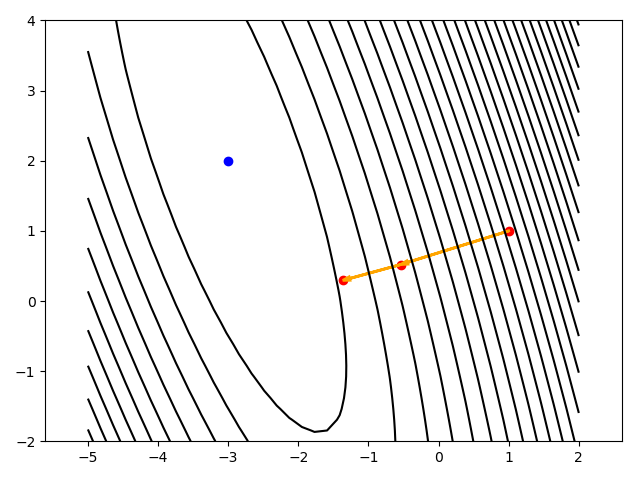
\includegraphics[scale=\myscale,scale=0.45]{figures/descente_pas_stochastique}
			\end{center}
		\end{minipage}
		\begin{minipage}{0.48\textwidth}
			\begin{center}
				{\bf Descente de gradient stochastique}
				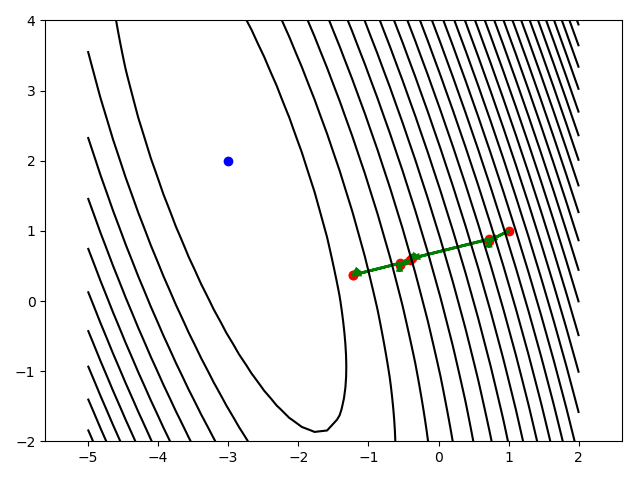
\includegraphics[scale=\myscale,scale=0.45]{figures/descente_stochastique}
			\end{center}
		\end{minipage}
	\end{center}
	
	
	Conclusion: sur cet exemple les points sont exactement sur la parabole d'équation $y=x^2+ax+b$ avec $a=-3$ et $b=2$. Bien sûr cette méthode est encore plus intéressante lorsqu'il s'agit de trouver une parabole qui ne contient pas l'ensemble des points donnés.
	\myfigure{1}{
		\tikzinput{fig-stochastique-02}
	}
	
\end{exemple}




Terminons par des remarques plus techniques.
Tout d'abord, la formule précise de la descente de gradient stochastique est :
$$P_{k+1} = P_k - \delta \grad E_{(k \% N)+1} (P_k)$$
où $k \% N$ est \og{}$k$ modulo $N$\fg{}.



La descente de gradient stochastique est une méthode qui peut être plus efficace : 
\begin{itemize}
	\item Tout d'abord elle n'utilise qu'une donnée à la fois et évite ainsi les problèmes de mémoire de la descente classique pour laquelle il faut manipuler toutes les données à chaque itération.
	\item Toujours dans le cas où l'on a beaucoup de données, la descente de gradient stochastique peut converger en deux ou trois passages sur l'ensemble des données, alors que la descente classique nécessite toujours plusieurs itérations (voir la section \ref{ssec:lot} plus loin).
	\item Avec la méthode stochastique, on calcule des gradients en des points qui sont plus proches du minimum. Attention cependant, certains petits pas peuvent aller dans la mauvaise direction.
	\item Le caractère aléatoire de ces petits pas est parfois un avantage, par exemple pour s'échapper d'un point-selle.
\end{itemize}






%--------------------------------------------------------------------
\subsection{Différentes fonctions d'erreurs}

Il existe différentes formules pour calculer l'erreur entre la sortie attendue $y_i$ et la sortie produite $F(x_i)$.

On considère une série de valeurs $y_i$, $i=1,\ldots,N$ (fournie par observations ou expérimentations) qui sont approchées par des valeurs $F(x_i)$ produites par une formule issue d'un réseau de neurones par exemple.
Le but est d'obtenir $F(x_i)$ le plus proche possible de $y_i$, pour tout $i=1,\ldots,N$. Pour savoir si l'objectif est atteint, on mesure l'écart entre ces valeurs.

\textbf{Erreur quadratique moyenne.}
$$E = \frac{1}{N} \sum_{i=1}^N (y_i-F(x_i))^2.$$

C'est la formule la plus classique (en anglais \emph{minimal squared error} ou \emph{mse}). 
Bien entendu $E\ge0$ quels que soit les $F(x_i)$ et $E=0$ si et seulement si $y_i=F(x_i)$ pour tous les $i=1,\ldots,N$. 
C'est presque la formule que l'on a utilisée pour la régression linéaire (il n'y avait pas le facteur $\frac1N$).

\textbf{Erreur absolue moyenne.}
$$E = \frac{1}{N} \sum_{i=1}^N |y_i-F(x_i)|.$$

C'est une formule plus naturelle, mais moins agréable à manipuler à cause de la valeur absolue.

Noter que pour ces deux formules, l'erreur globale $E$ est la moyenne d'erreurs locales $E_i = (y_i-F(x_i))^2$ (ou bien $E_i = |y_i-F(x_i)|$).
Les erreurs locales sont indépendantes les unes des autres, ce qui est la base de la descente de gradient stochastique.
(Une formule d'erreur du type $E = y_1y_2 - F(x_1)F(x_2)$ ne permettrait pas la descente stochastique.)

Il existe d'autres formules d'erreur, en particulier si la sortie attendue est du type $0$ ou $1$ ou bien si la sortie produite est une probabilité $0\le p \le 1$. 

% [[Ces formules seront détaillées dans la partie \og{}Statistique et probabilités\fg{}.]]

%--------------------------------------------------------------------
\subsection{Descente par lots}
\label{ssec:lot}

\index{descente de gradient!par lots}

Il existe une méthode intermédiaire entre la descente de gradient classique (qui tient compte de toutes les données à chaque itération)
et la descente de gradient stochastique (qui n'utilise qu'une seule donnée à chaque itération).

La descente de gradient par  \trouer{lots} (ou  \trouer{mini-lots}, \emph{mini-batch}) est une méthode intermédiaire : on divise les données par paquets de taille $K$. Pour chaque paquet (appelé \og{}lot\fg{}), on calcule un gradient et on effectue une itération.

Au bout de $N/K$ itérations, on a parcouru tout le jeu de données : cela s'appelle une  \trouer{époque}.
\index{descente de gradient!epoque@époque}


\myfigure{1.2}{
	\tikzinput{fig-epoque}
}

La formule est donc
$$P_{k+1} = P_k - \delta \grad (E_{j_0+1}+E_{j_0+2}+\cdots+E_{j_0+K}) (P_k).$$
Pour $P_{k+2}$, on repart de $P_{k+1}$ et on utilise le gradient de la fonction $E_{j_0+K+1}+E_{j_0+K+2}+\cdots+E_{j_0+2K}$.



	\begin{itemize}
		\item Pour $K=1$, c'est exactement la descente de gradient stochastique. Pour $K=N$, c'est la descente de gradient classique.
		
		\item Cette méthode combine le meilleur des deux mondes : la taille des données utilisées à chaque itération peut être adaptée à la mémoire et le fait de travailler par lots évite les pas erratiques de la descente stochastique pure.
		
		\item On peut par exemple choisir $2 \le K \le 32$ et profiter du calcul parallèle en calculant $\grad (E_1+\cdots + E_K)$, par le calcul de chacun des $\grad E_i$ sur $K$ processeurs, puis en additionnant les résultats.
		
		\item Il est d'usage de mélanger au hasard les données $(X_i,y_i)$ avant chaque époque.
	\end{itemize}




\begin{exemple}{}{}
	Voyons un exemple d'interpolation circulaire.
	Les $6$ points ci-dessous sont sur un cercle. Comment déterminer son centre et son rayon ?
	\begin{center}
		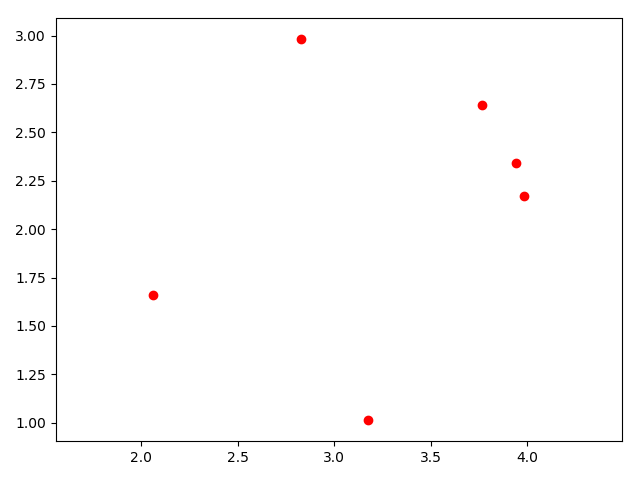
\includegraphics[scale=\myscale,scale=0.5]{figures/circulaire-01}
	\end{center}
	
	Pour des points $(x_i,y_i)$, $i=1,\ldots, N$, on mesure la distance globale par rapport au cercle $\mathcal{C}$ de centre $(a,b)$ et de rayon $c$ par la formule d'erreur :
	$$E(a,b,c) = \sum_{i=1}^N E_i(a,b,c)$$
	où 
	$$E_i(a,b,c) = \big( (x_i-a)^2 + (y_i-b)^2 - c^2 \big)^2.$$
	En effet, $E_i$ mesure en quelque sorte la distance entre le point $(x_i,y_i)$ et le cercle $\mathcal{C}$ de centre $(a,b)$ et de rayon $c$. Donc $E_i=0$ si et seulement si $(x_i,y_i) \in \mathcal{C}$, sinon $E_i > 0$.
	
	\myfigure{1}{
		\tikzinput{fig-circulaire-01}
	}
	
	Dans notre exemple, les $N = 6$ points sont exactement situés sur le cercle de centre $(a,b)$ et de rayon $c$. En appliquant la descente de gradient par lots avec $\delta = 0.01$ et $(a_0,b_0,c_0) = (1,1,2)$, on trouve $(a,b) = (3,2)$ et $c=1$.
	Ci-dessous, à droite, nous avons représenté les valeurs de l'erreur totale $E$ (qui tend vers $0$) en fonction du nombre d'époques et ceci pour différentes tailles du lot : $K=1$ (descente stochastique), $K=2$, $K=3$ et $K=6$ (descente classique).
	\begin{center}
		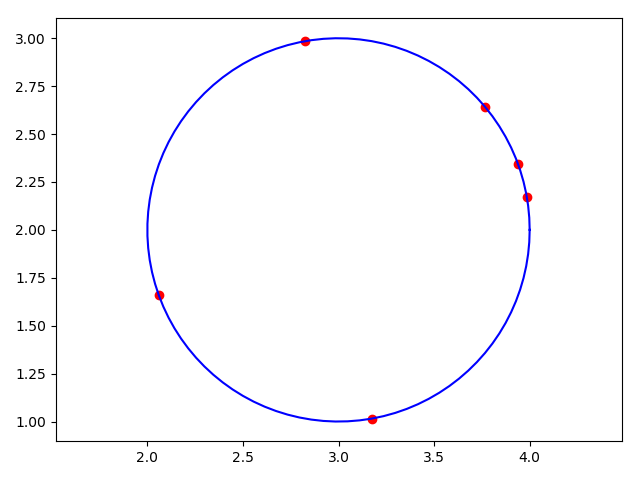
\includegraphics[scale=\myscale,scale=0.5]{figures/circulaire-02}
		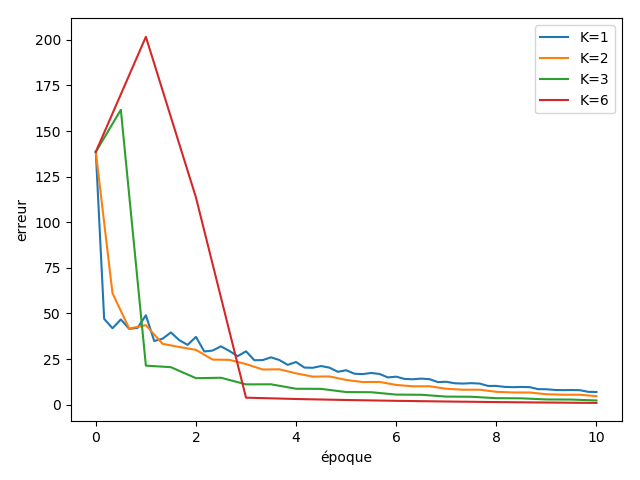
\includegraphics[scale=\myscale,scale=0.5]{figures/circulaire-03}
	\end{center}
	On remarque qu'au bout de $10$ époques la valeur de l'erreur est à peu près la même quelle que soit la taille $K$ de l'échantillon. Par contre, l'évolution au départ est différente. Par exemple pour $K=1$, l'erreur fluctue à la hausse ou à la baisse à chaque itération. 
	
	Cette méthode présente bien sûr davantage d'intérêt quand les points ne sont pas exactement sur un cercle. Il s'agit alors de trouver le meilleur cercle qui convient, c'est-à-dire de trouver le minimum (cette fois non nul) de $E$.
	Voici un exemple de $N = 100$ points tirés au hasard autour du cercle de centre $(a,b) = (1,2)$ et de rayon $c=3$.
	La descente de gradient est appliquée avec $\delta = 0.001$ et $(a_0,b_0,c_0) = (1,1,1)$ pour des lots de différentes tailles $K=1$, $K=10$ et $K=20$. On remarque que deux époques suffisent pour avoir convergence et que plus la taille $K$ de l'échantillon est grande plus la convergence est régulière vers le minimum.
	
	\begin{center}
		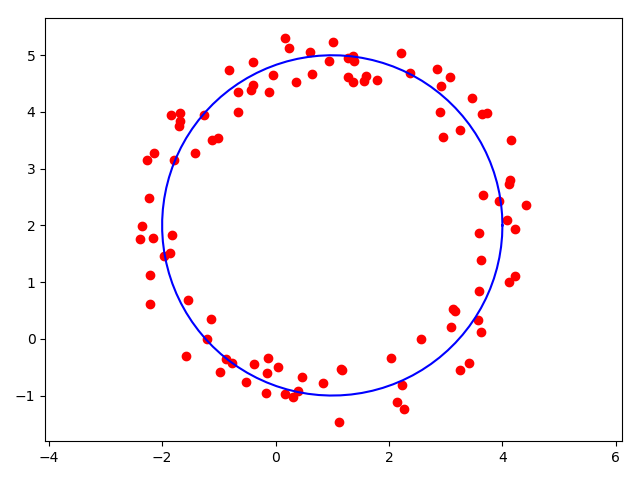
\includegraphics[scale=\myscale,scale=0.5]{figures/circulaire-04}
		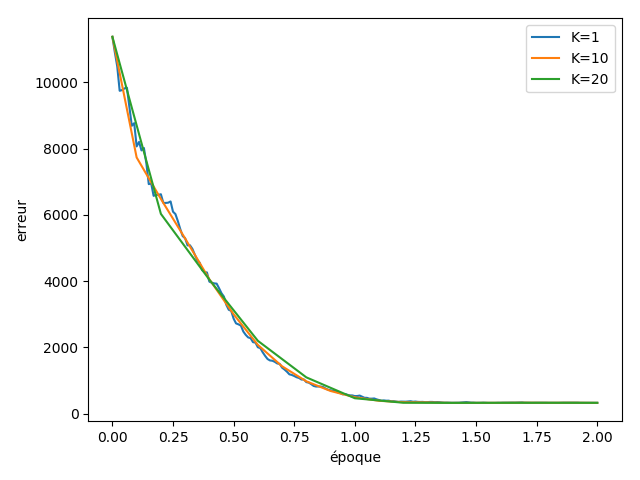
\includegraphics[scale=\myscale,scale=0.5]{figures/circulaire-05}
	\end{center}
	
\end{exemple}

%%%%%%%%%%%%%%%%%%%%%%%%%%%%%%%%%%%%%%%%%%%%%%%%%%%%%%%%%%%%%%%%%%%%%
\section{Accélérations}


Le choix du pas $\delta$ n'est pas la seule amélioration possible de la méthode du gradient, nous allons voir comment la modifier à l'aide du \og{}moment\fg{}. Commençons par revenir à l'analogie de la descente du gradient classique qui correspond à une goutte d'eau qui descend une montagne : la goutte emprunte le chemin qui suit la courbe de plus grande pente, quitte à serpenter et osciller lors de la descente. Imaginons que l'on lance maintenant une balle assez lourde du haut de la même montagne. Cette balle va suivre, comme la goutte d'eau, le chemin de la plus forte pente, mais une fois lancée elle va acquérir de l'inertie, appelée  \trouer{moment}, qui va atténuer ses changements de direction.
Ainsi la balle ne s'embarrasse pas des petits aléas du terrain et dévale la pente plus rapidement que la goutte d'eau.


Nos petits aléas de terrain à nous viennent du fait que l'on ne calcule pas exactement le gradient de la fonction d'erreur en utilisant tout le jeu de données à chaque fois, mais seulement un échantillon. Cela peut conduire à certains gradients mal orientés. L'inertie de la balle est en quelque sorte la mémoire de la trajectoire passée qui corrige les mouvements erratiques.

Sur la figure de gauche, la descente classique (la goutte d'eau), sur la figure de droite, la descente de gradient avec le moment (la balle).

\myfigure{1}{
	\tikzinput{fig_moment01}\qquad\qquad 
	\tikzinput{fig_moment02}
}

%--------------------------------------------------------------------
\subsection{Moment}

\index{descente de gradient!moment}

Rappelons la formule de la descente de gradient classique :
$$P_{k+1} = P_k - \delta \grad f(P_k).$$

\myfigure{1}{
	\tikzinput{fig_moment03}
}

Considérons nos points comme une particule qui voyage au cours du temps. Alors
le vecteur $\overrightarrow{P_{k-1}P_k}$ correspond à la vitesse de cette particule et est appelé le  \trouer{moment} au point $P_k$.

La formule de la descente de gradient avec moment est :
$$P_{k+1} = P_k + \mu\overrightarrow{P_{k-1}P_k}  - \delta \grad f(P_k).$$
où $\mu,\delta \in \Rr$. Cette formule peut être définie pour $k=0$ si on suppose que la particule est immobile au départ, c'est-à-dire en posant $\overrightarrow{P_{-1}P_0} = \vec 0$.

On peut prendre par exemple $\mu \in [0.5,0.9]$ et $\delta = 0.01$.


Schématiquement, au point $P_k$ nous avons deux vecteurs : un qui provient du moment $\mu\overrightarrow{P_{k-1}P_k}$ (la mémoire du passé) et un qui provient du gradient $- \delta \grad f(P_k)$ (qui projette vers l'avenir). La somme permet de calculer le point suivant  $P_{k+1}$.

\myfigure{1.2}{
	\tikzinput{fig_moment04}
}





%--------------------------------------------------------------------
\subsection{Nesterov}

\index{descente de gradient!acceleration de Nesterov@accélération de Nesterov}

Dans la méthode précédente, le moment et le gradient sont calculés au même point $P_k$. La méthode de Nesterov est une variante de cette méthode. 
Elle consiste à appliquer d'abord le moment, pour obtenir un point $P_k'$, puis de calculer le gradient en ce point (et non en $P_k$).

La formule est donc 
$$P_{k+1} = P_k + \mu\overrightarrow{P_{k-1}P_k}  - \delta \grad f(P_k+\mu\overrightarrow{P_{k-1}P_k}).$$
Autrement dit, si on note $P_k'$ le point $P_k + \mu\overrightarrow{P_{k-1}P_k}$ alors
$$P_{k+1} = P_k'  - \delta \grad f(P_k').$$

\myfigure{1.2}{
	\tikzinput{fig_moment05}
}


C'est un petit avantage par rapport à la méthode du moment puisqu'on calcule le gradient au point $P_k'$ qui est censé être plus près de la solution $P_{\min}$ que $P_k$.


%--------------------------------------------------------------------
\subsection{Vocabulaire}

Terminons par un petit résumé du vocabulaire avec sa traduction en anglais :
\begin{itemize}
	\item descente de gradient (classique), \emph{(batch) gradient descent},
	\item descente de gradient stochastique, \emph{sgd} pour \emph{stochastic gradient descent},
	\item descente de gradient par lots, \emph{mini-batch gradient descent},
	\item pas $\delta$, \emph{learning rate},
	\item erreur quadratique moyenne, \emph{mse} pour \emph{minimal squared error},
	\item moment, \emph{momentum},
	\item époque, \emph{epoch}.
\end{itemize}  
